\chapter{Introduction and Definition of Terms}

\begin{table}[h!t]
\caption{These are some of the commonly used notations for this work.  Most of the non-standard notation is introduced and explained in dedicated sections of the introduction chapter, but this table is a quick reference for the sets and spaces used throughout.}
\label{tab:note}

\begin{tabular}{c|cp{9cm}}
\cb &
\cb & 
\cb Meaning 
    \upstrut{4mm}
    \\
\cw \multirow{4}{*}{{\bf SETS}}&\cw $\mathbb{C}$ &\cw set of all complex numbers\\
&\cy $\mathbb{R}$ &\cy set of all real numbers\\
&\cw $\mathbb{R_+}$ &\cw set of all positive real numbers\\
&\cy $\mathbb{Z}$ &\cy set of all integers\\
\hline
\cw \multirow{5}{*}{ {\bf SPACES}}&\cw $\mathcal{H}^S$ &\cw reduced system Hilbert space\\
&\cy $\mathcal{H}^B$ &\cy bath Hilbert space\\
&\cw $\mathcal{H}^{SB}$ &\cw composite system Hilbert space\\
&\cy $\mathcal{S}(\mathcal{H}^X)$ &\cy set of all valid density matrices on the Hilbert space called $X$\\
&\cw $\mathcal{B}(\mathcal{H}^X)$ &\cw set of all bounded operators on the Hilbert space called $X$\\
\hline
\cw \multirow{4}{*}{{\bf OPERATIONS}}&\cy $\trace$ &\cy trace of an operator or matrix\\
&\cw $\sharp$ &\cw assignment of composite system states to reduced system states(see Sec.\ \ref{sec:sharpop})\\
&\cy $\flat$ &\cy partial trace over the bath (see Sec.\ \ref{sec:parttrace}\\
&\cw $\mathbf{A}\odot$ &\cw ``constructor'' called $A$ that takes vectors of states to other objects, e.g.\ matrices (see Sec.\ \ref{sec:notation})\\
\hline
\end{tabular}
\end{table}


\section{Motivation}

A ``quantum operation'' was originally introduced in 1961 with a discussion of the stochastic dynamics of quantum systems \cite{Sudarshan1961}.  Quantum operations have become increasingly important as sub-fields of quantum information move towards experimental verification of key concepts and technologies.  In quantum information theory, quantum operations are called ``quantum channels'' and are formally represented by linear, trace-preserving, completely positive maps (commonly abbreviated as ``CPTP'').  The ``completely positive'' qualifier in the definition of a quantum channel can be removed.  Such channels are called ``negative channels'' and are the topic of this work.  A negative quantum channel (or quantum operation) is mathematically represented by a linear, trace-preserving map with a consistent assignment of reduced system states to composite system states.  It will be shown that the complete positivity requirement is not necessary and may, in many cases, not be a valid physical assumption.  

We will use the tools of open quantum systems and quantum information.  The theory of open quantum systems provides the most general framework for discussions of quantum dynamics, and quantum information theory provides useful concepts that will help make the discussion more lucid.  Several concepts from quantum information will be used without modification (such as qubits\footnote{Qubits are ideal quantum mechanical systems consisting of only two states.  The name harkens back to information theory roots, but the concept of a ``two level atom'' is a well established and very popular theoretical tool in physics.}), but many other concepts will be redefined.  All such redefinitions will be discussed as they are presented.  The popularity of quantum information plays a major role in our motivation; hence, most of the examples will be taken from sub-fields such as quantum computing and quantum communication.

The study of open quantum systems can be traced back to Von Neumann \cite{vonNeumann1947} and originally came about in the study of the thermodynamics of non-equilibrium systems.  The field gained popularity in studies of quantum foundations as a way to understand decoherence and related concepts such as the ``quantum-classical'' divide.  Currently, open systems are enjoying yet another resurgence in popularity as the formalism is applied to simple quantum systems used in quantum information theory.  The problem of noise in quantum information is considered somewhere between a serious problem and the reason quantum technologies will ultimately fail to be practical (or even experimentally verified in some cases).  As such, traditional open system concepts (e.g.\ spin baths, spin-boson models, Lindblad evolutions, etc) have become quite important to the study of quantum information.

We will begin with a very brief introduction to open quantum systems from the quantum information frame of reference.  The discussion will then turn to complete positivity and its ubiquitousness in the quantum information literature.  We will close with discussions of quantum operations that are not completely positive including examples, implications, and utilities.  

\section{Open Systems}
An open quantum system is a quantum system which is coupled to another quantum object (usually called the ``bath'', ``environment'', or ``reservoir'').  A simple sketch of such a system is given  in Fig. \ref{fig:sysbathdiagram}.

\begin{figure}[t!]
    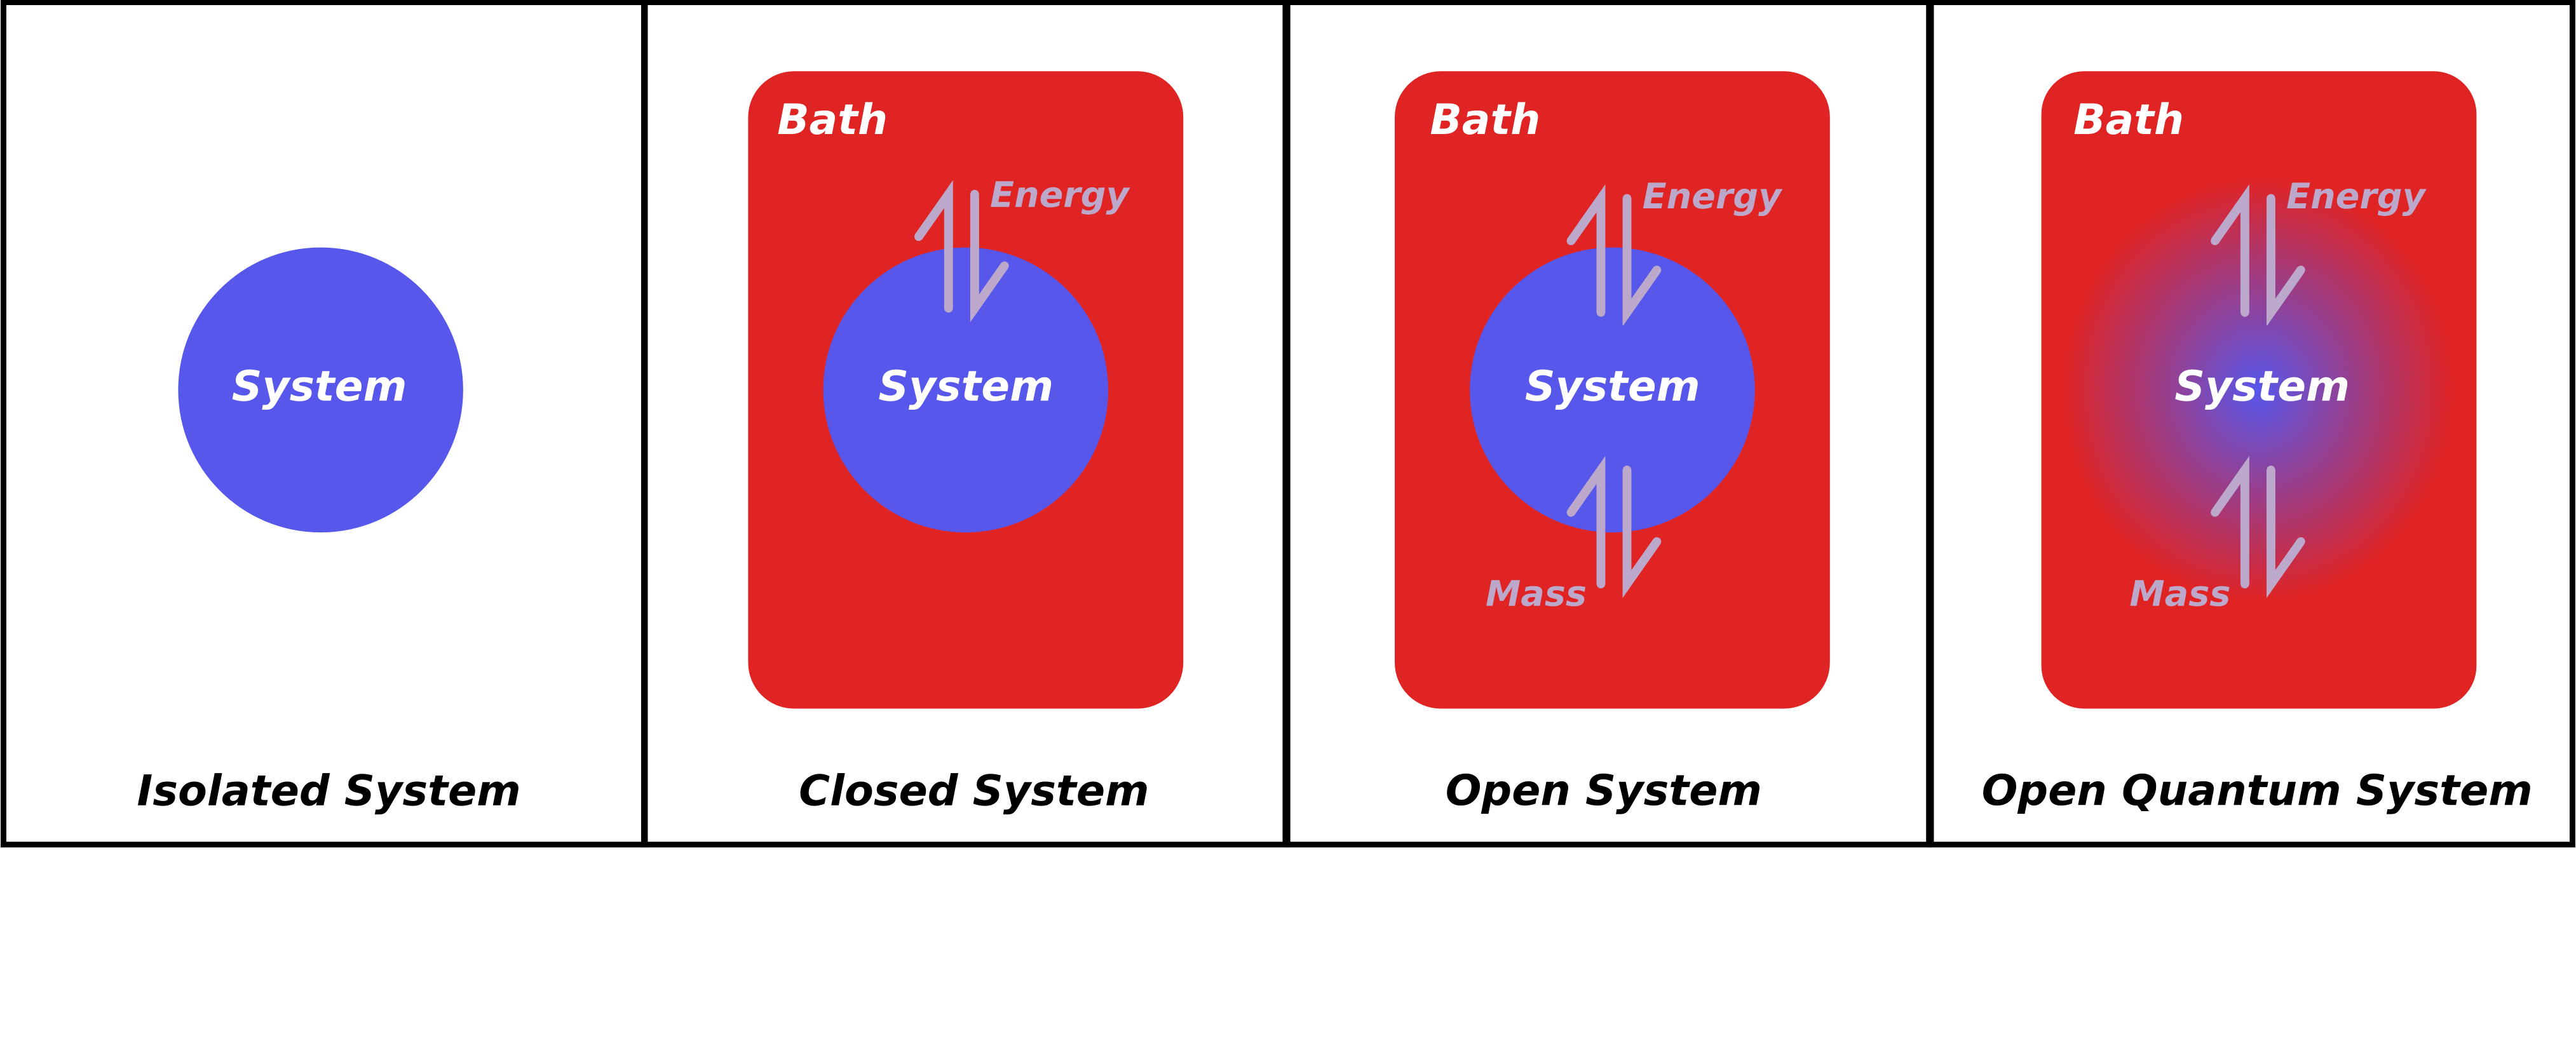
\includegraphics[scale=0.65]{OpenSystemDiagram.png}
  \caption{An ``isolated'' system is a system without any kind of bath, a ``closed'' system has a bath with which it can exchange energy (e.g.\ heat and work), an ``open'' system has a bath with which it can exchange both energy and matter, and an ``open quantum'' system has a bath with which it can exchange energy and matter but with which the boundary is not clearly defined.  See the text for further discussion of the system-bath boundary in an open quantum systems.  Notice that these definitions apply to non-relativistic systems; see \cite{Breuer2007} for a discussion of open quantum systems and relativity.}
  \label{fig:sysbathdiagram}
\end{figure}

The system of interest (called ``system'' in the diagram; also called the ``reduced system'') is a subsystem of the combined system (called the ``composite system''). The composite system is assumed to be closed and follows Hamiltonian dynamics.  The interactions between the reduced system and the bath lead to dynamics of the reduced system which include correlations and coupling between the two subsystems.  As a result, the reduced system will, in general, no longer follow unitary Hamiltonian dynamics.   

The idea of a quantum system-bath setup is very similar to the traditional ideas of open systems in thermodynamics.  The reduced system is free to interact with the environment in any way.  Heat, particles, entropy, etc.\ can all be exchanged across the system-bath interface exactly as in thermodynamics.  The difference here is that the system may also become entangled with the bath.  This system-bath entanglement will lead to dynamics that are not studied in thermodynamics, and the entanglement with the bath is considered by many to be the primary source of decoherence in experiments \cite{Zurek2003}.

Formal definitions of the reduced system and the bath are disputed.  ``Open systems'' exist in many different fields outside of physics, including computing and social sciences (e.g.\ \cite{Luhmann1995}), and the general definition is always the same: an ``open system'' is a system influenced by its environment.  In open quantum systems, however, there is a question of system delineation.  For example, suppose the reduced system is a single electron and the bath is every other electron in some heterostructure in an experiment.  It seems simple enough to call the electron the ``reduced system'' because it is the focus of the experiment (i.e.\ it is the ``system of interest'').  However, this definition introduces the experimenter into the definition of the reduced system.  This definition could be rephrased as ``the electron is the reduced system because the experimenter wants it to be the reduced system''.  Of course, there is nothing wrong with such a definition, but it might not be philosophically or foundationally satisfying.  Suppose the electron is entangled with every other electron in the heterostructure.  Can the electron now still be considered the reduced system simply because the experimenter wishes it?  Does the entanglement between the single electron and the sea of electrons in the structure completely blur the reduced system-bath boundary?  Perhaps the entanglement requires all the electrons in the system to be considered the reduced system together.  Perhaps the standard approach and definitions for open quantum system do not apply to highly entangled systems.

Such foundational issues are outside the scope of this discussion, so we will adhere to a strict definition of ``reduced system''.  
\begin{definition}
The {\em reduced system} is the part of the experiment directly accessible (e.g.\ through measurements and preparations) by the experimenter.  
\end{definition}

See Appendix \ref{sec:redsysdef} for a discussion of this definition.  In the example above, the single electron would be called the reduced system if it is the only electron in the system under the control of the experimenter.  Naturally, the bath is then defined as the part of the experiment inaccessible to the experimenter.  This definition is a straightforward, physical way to divide the open system under investigation.  If a qubit is constructed from a double quantum dot system, then the double quantum dot system is the reduced system because the experimenter has a way to control it.  The phonon bath that impairs the performance of that qubit is the bath because the experimenter has no way to control it.  The experimenter might really want that phonon bath to be part of his reduced system, but he is always restricted by his technological capabilities\footnote{This restriction is often pointed out by proponents of open systems theories with the platitude ``There is no such thing as a closed quantum system.''}.

\section{Density Matrix}
\label{sec:densitymatrix}
The state of a system will be described by a density matrix rather than a state vector \cite{vonNeumann1947,Landau1977,blum1996}.  Suppose the experimenter has some classical uncertainty about the state of a system.  Classical uncertainty is the experimenter's ignorance as to the state of the system given several different possible states of the system\footnote{Classical uncertainty can be contrasted with quantum uncertainty which is a fundamental limit to the precision of simultaneous measurements of conjugate variables of the system (e.g.\ position and momentum).  See \cite{Sakurai2010} for a discussion of the quantum uncertainty principle.}.  For example, he might know the system is in some pure state $|\varphi_i\rangle$ with probability $p_i$ given $\sum_i p_i =1$.  He would then need to take a classical average of quantum expectation values to find the total expectation value for his experiment, i.e.
$$
\langle A\rangle = \sum_i p_i \langle\varphi_i |A|\varphi_i\rangle\;\;.
$$
The density matrix is defined as
$$
\rho := \sum_i p_i |\varphi_i\rangle\langle\varphi_i|\;\;.
$$
Hence, the expectation value of an operator can be written in terms of the density matrix as
$$
\langle A\rangle = \trace(\rho A)\;\;.
$$
The following properties follow directly from the definition:
$$\trace(\rho) = 1\;\;,$$
$$\rho^\dagger=\rho\;\;,$$
$$\rho\ge 0\;\;,$$
$$\trace(\rho^2) = 1 \Rightarrow \textrm{pure state}\;\;,$$
where a ``pure state'' is defined as a state that can be represented by a state vector (i.e.\ $\rho = \ketbra{\phi}{\phi}$ for some state vector $\ket{\phi}$).  The probability of measuring a state $\rho$ in the state $|\phi\rangle$ is the expectation value of the operator $|\phi\rangle\langle\phi|$; i.e.
\begin{eqnarray}
P_\phi &=& \trace(\rho |\phi\rangle\langle\phi|) \\
&=& \langle\phi|\rho|\phi\rangle
\end{eqnarray}
Hence, the probability of distinguishing a particular state can be phrased as ``measuring the projector'' of that particular state.


The positivity requirement for the density matrix
$$
\langle \psi |\rho |\psi \rangle \ge 0\;\forall \ket{\psi} \;\;,
$$
(where $\ket{\psi}$ is some pure state) written as $\rho \ge 0$, insures the eigenvalues of $\rho$ are all positive semi-definite.  The unit trace requirement 
$$
\trace(\rho) = 1
$$
insures all the eigenvalues sum to 1.  These two requirements allow the eigenvalues of $\rho$ to be interpreted as formal probabilities, i.e.\ each eigenvalue is a real number between zero and one, and all the eigenvalues sum to one.  

The self-adjoint property for $\rho$ (which is implied by the positivity \cite{Eidelman2004}) is the final lynch pin in the statistical interpretation of the density matrix.  All observables in quantum mechanics are represented as linear, self-adjoint operators.  
\begin{definition}
A {\em self-adjoint operator} is an operator that is its own adjoint.  The matrix representing a self-adjoint operator is Hermitian \cite{Byron1992}, i.e.\ it is equal to its conjugate transpose.  We will only be dealing with finite dimensional systems, so self-adjoint operators for us will mean operators with a Hermitian matrix representation.
\end{definition}

The state $\rho$ can be shown to be Hermitian, but the self-adjoint requirement extends to all observables.  A self-adjoint operator can be decomposed using the spectral theorem into an orthonormal basis, and the operator will have a diagonal matrix representation on this basis (see \cite{Nielsen2010} for a discussion of the spectral decomposition of the density matrix and see \cite{Breuer2007} for a more complicated discussion of the spectral theorem for operators in the general case).  The measurement postulate of quantum mechanics is formulated in terms of projection operators.  Projection operators cannot be used to find the off-diagonal matrix elements of the matrix representation of an operator.  Notice that if an observable could not be diagonalized in some basis then the operator would always contain some information that was inaccessible to the experimenter by direct observation (i.e. ``measurement'').

\section{Mathematical Structure of Open Systems}

\subsection{System State Spaces}
A quantum system in a pure state can be represented by some state vector $S$ in a Hilbert space $\mathcal{H}^S$.  A possibly mixed (i.e.\ not pure) state of the system will be represented by some density operator $\rho^S\in \mathcal{S}(\mathcal{H}^S)$.  The set $\mathcal{S}(\mathcal{H}^X)$ is the set of all valid states $\rho$ in the Hilbert space space labeled $X$, and the set $\mathcal{B}(\mathcal{H}^X)$ is the set of all bounded operators in $X$.  This notation will be important in later discussions when it is applied to both the reduced system and the bath Hilbert spaces.

The state of the composite system is defined in a tensor product Hilbert space $\mathcal{H}^S\otimes\mathcal{H}^B$ where $\mathcal{H}^S$ is the Hilbert space of the reduced system and $\mathcal{H}^B$ is the Hilbert space of the bath.  The reduced system will have some state
$$
\rho^S\in\mathcal{S}(\mathcal{H}^S)\;\;,
$$
the bath will have some state
$$
\rho^B\in\mathcal{S}(\mathcal{H}^B)\;\;,
$$
and the composite system will have some state
$$
\rho^{SB}\in\mathcal{S}(\mathcal{H}^{SB})\;\;.
$$
The relationship of the composite system to its component states will be important and is referred to as the system-bath correlation.  A product state is defined by the following relationship:
$$
\rho^{SB} = \rho^{S}\otimes\rho^{B}\;\;,
$$
where $\rho^S\in\mathcal{S}(\mathcal{H}^S)$ and $\rho^B\in\mathcal{S}(\mathcal{H}^B)$.  If the state is not a product state, it might still be a separable state, i.e.\ it might have the form
$$
\rho^{SB} = \sum_{ij} p_{ij} \rho^{S}_i\otimes\rho^{B}_j\;\;,
$$
where $\rho^S_i\in\mathcal{S}(\mathcal{H}^S)$, $\rho^B_j\in\mathcal{S}(\mathcal{H}^B)$, $p_{ij}\ge0\;\forall i,j$ and $\sum_{ij} p_{ij}=1$. The set of separable states of the composite system will be denoted $\mathcal{G}^{SB}$.  Notice if $\rho^{SB}$ is a product state then $\rho^{SB}\in\mathcal{G}^{SB}$, but the converse is not necessarily true.  The composite state is entangled if and only if it is not separable.  

\subsection{Partial Trace}
\label{sec:parttrace}
The relationship between the states of the subsystems and the composite system can be defined by looking at expectation values.  The {\em partial trace} will be defined as the operation that ensures consistent measurement statistics between an observable and its trivial extension to a higher dimensional space.

The trivial extension of an operator is an operator that acts on any extended space as the identity operator.  Let $A\in\mathcal{B}(\mathcal{H}^X)$ be an observable with the trivial extension $\tilde{A}=A\otimes I\in\mathcal{B}(\mathcal{H}^{XY})=\mathcal{B}(\mathcal{H}^X\otimes\mathcal{H}^Y)$ where $I$ is the identity operator.  In this example, $A$ acts on space $X$, so it's trivial extension, $\tilde{A}$, acts on the extended space, $Y$, as identity.

If $\{\ket{x_i}\}$ is a basis of $\mathcal{H}^X$ and $\{\ket{y_j}\}$ is a basis of $\mathcal{H}^Y$, than $\{\ket{x_i}\otimes\ket{y_j}\equiv\ket{x_iy_j}\}$ is a basis of $\mathcal{H}^{XY}$.  A few more definitions are required to completely define this experiment: $\rho^X\in\mathcal{S}(\mathcal{H}^X)$, $\rho^Y\in\mathcal{S}(\mathcal{H}^Y)$, and $\rho^{XY}\in\mathcal{S}(\mathcal{H}^{XY})$ are the states of subsystem $X$, subsystem $Y$, and their joint $XY$ system, respectively.

The expectation value of $A$ is given by
\begin{eqnarray*}
\mean{A} &=& \trace(\rho^X A)\\
&=& \sum_i \bra{x_i}\rho^X A\ket{x_i}\;\;, 
\end{eqnarray*}
and it is assumed that this value should be equal to $\mean{\tilde{A}}$.  The observable $\tilde{A}$ acts on the joint $XY$ system and is defined as the operation of $A$ on subsystem $X$ and ``nothing'' on subsystem $Y$.  The joint $XY$ system is defined to have subsystems $X$ and $Y$, and $I$ is defined as the operator which leaves a system unchanged.  Hence, $\mean{A}=\mean{\tilde{A}}$ is a justified assumption\footnote{It can be argued that the extension of $A$ to the joint $XY$ system is not $A\otimes I$.  It might even be argued that such an extension is not possible \cite{Gisin2001}, i.e.\ it might be argued that trivial extensions are not valid physical concepts.  Such an argument, however, invalidates the definition of the partial trace and has the logical extension of requiring the theorist to take the entire quantum universe into account in the calculation of $\mean{A}$.}.

The expectation value of $\tilde{A}$ is given by
\begin{eqnarray*}
\mean{\tilde{A}} &=& \trace(\rho^{XY} \tilde{A})\\
&=& \sum_{mn} \bra{x_my_n}\rho^{XY} \tilde{A}\ket{x_my_n}\;\;.
\end{eqnarray*}
Inserting the identity operator on the joint $XY$ system, $I^{XY}=\sum_{ij}\ketbra{x_iy_j}{x_iy_j}$, into the above equation yields
\begin{eqnarray*}
\mean{\tilde{A}} &=& \sum_{mnij} \bra{x_my_n}\rho^{XY} \ketbra{x_iy_j}{x_iy_j}\tilde{A}\ket{x_my_n}\\
&=& \sum_{mnij} \bra{x_my_n}\rho^{XY} \ket{x_iy_j} \bra{x_i}A\ket{x_m}\braket{y_j}{y_n}\\
&=& \sum_{mij} \bra{x_my_j}\rho^{XY} \ket{x_iy_j} \bra{x_i}A\ket{x_m}\;\;.
\end{eqnarray*}
Notice, $\sum_j \bra{x_my_j}\rho^{XY} \ket{x_iy_j}$ are matrix elements of some new state.  For convenience, we call this new state $\rho^?$.  Notice that $\rho^?$ is defined in terms of $\rho^{XY}$ and is independent of $\mathcal{H}^Y$ because of the sum over the basis $\{y_j\}$.  The state $\rho^?$ is literally the result of ``tracing out'' subsystem $Y$ from the joint system $XY$, i.e.\ $\bra{x_k}\rho^?\ket{x_l}=\sum_h \bra{x_ky_h}\rho^{XY}\ket{x_ly_h}$.  

Using this new notation, the expectation value becomes
\begin{eqnarray*}
\mean{\tilde{A}} &=& \sum_{mi} \bra{x_m}\rho^{?} \ket{x_i} \bra{x_i}A\ket{x_m}\\
&=& \sum_{m} \bra{x_m}\rho^{?} A\ket{x_m}\\
&=& \trace\left( \rho^{?} A\right)\;\;,
\end{eqnarray*}
where $\sum_i \ketbra{x_i}{x_i} = I\in\mathcal{B}(\mathcal{H}^X)$ was used.  

The original assumption was that 
$$
\mean{A}=\mean{\tilde{A}}\;\;,
$$
which can be rewritten using the above results as
$$
\trace\left(\rho^X A\right) = \trace\left( \rho^{?} A\right)\;\;.
$$
From this form of the original assumption, it can be seen that if $\rho^? = \rho^X$, then $\mean{A}=\mean{\tilde{A}}$.

The matrix elements of the subsystem states (in the $\{\ket{x_i}\}$ basis) are defined in terms of the composite states as
$$
\bra{x_k}\rho^X\ket{x_l}=\sum_h \bra{x_ky_h}\rho^{XY}\ket{x_ly_h}
$$
and
$$
\bra{y_k}\rho^Y\ket{y_l}=\sum_h \bra{x_hy_k}\rho^{XY}\ket{x_hy_l}\;\;.
$$
The subsystem states are written more succinctly as $\rho^X = \trace_Y(\rho^{XY})$ and $\rho^Y = \trace_X(\rho^{XY})$.  The operation $\trace_X(\rho^{XY})$ is called the {\em partial trace} with respect to $X$ or ``tracing out'' subsystem $X$.  This operation is normally introduced in physics texts in the manner it has been presented here \cite{Cohen1992,Nielsen2010,Jacobs2013,Barnett2002}, but the same partial trace presented above can be defined in a basis-independent fashion \cite{Carlen2010}.  

The partial traces preserves the trace of the reduced system, i.e.\
$$
\trace\left(\rho^X\right) = \sum_i \bra{x_i}\rho^X\ket{x_i} = \sum_{hi} \bra{x_iy_h}\rho^{XY}\ket{x_iy_h} = \trace\left(\rho^{XY}\right)\;\;,
$$
where the second to last equality follows from the definition of the matrix elements of subsystem state in terms of the composite state.  This result shows that $\trace\left(\rho^{XY}\right)=1\Rightarrow\trace\left(\rho^X\right)=1$ if $\rho^X = \trace_Y\left(\rho^{XY}\right)$.  It can also be shown that $\rho^{XY} = \left(\rho^{XY}\right)^\dagger\Rightarrow \rho^{X} = \left(\rho^{X}\right)^\dagger$ and $\rho^{XY}\ge 0\Rightarrow \rho^{X}\ge 0$ if $\rho^X = \trace_Y\left(\rho^{XY}\right)$ \cite{Paris2012}.  Hence, if $\rho^{XY}$ is a valid density operator and $\rho^X$ is defined using the partial trace as $\trace_Y\left(\rho^{XY}\right)$, then $\rho^X$ will also be a valid density operator.

The partial trace ensures consistency between measurements on the reduced system and the trivial extension of such measurements to the composite system.  As such, the introduction of the partial trace leads directly to the definitions of the reduced system and bath states.
\begin{definition}
The state of the reduced system (called the {\em reduced density matrix} or {\em reduced state}) is defined as
$$
\rho^S:=\trace_B(\rho^{SB})\;\;,
$$
and the (much less frequently used) state of the bath is defined as
$$
\rho^B:=\trace_S(\rho^{SB})\;\;.
$$
\end{definition}

The partial trace with respect to the bath is a very common operation in the study of open systems, and, for that reason, we will use special notation for tracing out the bath: If $\tau\in\mathcal{S}(\mathcal{H}^{SB})$, then $\tau^\flat\in\mathcal{S}(\mathcal{H}^S)$.  
\begin{definition}
The {\em flat operator} is equivalent to the partial trace with respect to the bath, i.e.\ $\tau^\flat\equiv\trace_B(\tau)$.  
\end{definition}

The reduced state is written down in this notation as
$$
\rho^S = (\rho^{SB})^\flat\;\;.
$$
The utility of this notation will become clear in the the following sections.  

\subsection{Assignments of Subsystem States}
\label{sec:sharpop}

In general, a complete understanding of the behavior of the reduced system would require knowledge of the composite state.  Unfortunately, the reduced system state is defined in terms of the composite state through the use of a non-invertible operation, the partial trace.  By definition, the reduced system is the only part of the open system accessible to the experimenter, so how is the experimenter to know $\rho^{SB}$?  

This problem has been addressed by Pechukas and Alicki with the introduction of an assignment map \cite{Pechukas1994}\cite{Alicki1995}\cite{Pechukas1995}.  The assignment map\footnote{It should be noted that the term ``map'' is used throughout the literature, but it is not always clear that the object being discussed is a mathematically well defined map (e.g.\ see \cite{Fraleigh2003} for a basic definition of a map).} acts as a kind of inverse to the partial trace.  For example, define an assignment map $A$ that acts such that if $\tau\in\mathcal{S}(\mathcal{H}^S)$ then
$$
A(\tau)\in\mathcal{S}(\mathcal{H}^{SB})\;\;.
$$
Such a construction leads to some interesting conceptual problems.  For example, consider the set of two qubit Bell states
\begin{eqnarray*}
\ket{B_0} = \frac{\ket{00}+\ket{11}}{\sqrt{2}}\;\;,\\
\ket{B_1} = \frac{\ket{00}-\ket{11}}{\sqrt{2}}\;\;,\\
\ket{B_2} = \frac{\ket{01}+\ket{10}}{\sqrt{2}}\;\;,
\end{eqnarray*}
and
$$
\ket{B_3} = \frac{\ket{01}-\ket{10}}{\sqrt{2}}\;\;.
$$
One of the two qubits in the above states can be defined as the bath, which leads to
$$
(\ketbra{B_0}{B_0})^\flat = (\ketbra{B_1}{B_1})^\flat = (\ketbra{B_2}{B_2})^\flat = (\ketbra{B_3}{B_3})^\flat = \frac{I}{2}\;\;.
$$
Define a reduced state $\tau\in\mathcal{S}(\mathcal{H}^{S})$ and composite state $\rho\in\mathcal{S}(\mathcal{H}^{SB})$ such that 
\begin{equation}
\label{eqn:rhotau}
\rho^\flat = \tau\;\;.
\end{equation} 
If $\tau = I/2$, Eqn.\ \ref{eqn:rhotau} would be satisfied if the composite state $\rho$ was any of the Bell states, and it would not be possible to determine the specific Bell state of $\rho$ with knowledge of $\tau$ alone.  

The assignment operation could be constructed as
$$
A(\tau) = \Gamma\;\;,
$$
where
$$
\Gamma = \{\rho\in\mathcal{S}(\mathcal{H}^{SB})\;|\;\rho^\flat = \tau\}\;\;,
$$
i.e.\ the assignment operator could produce a set of composite states, each of which obeys the expected behavior of Eqn.\ \ref{eqn:rhotau}.  Such a construction quickly runs into problems.  For example, suppose $A$ is linear and $\tau=\sum_i p_i \tilde{\tau}_i$.  The assignment of $\tau$ would be
$$
A(\tau) = \sum_i p_i A(\tilde{\tau}_i)\;\;,
$$
but now there is the problem of defining the addition of sets of composite states.  Furthermore, the utility of this construction would require some kind of average over a set of composite states.  

Discussions of assignment maps in the literature center around discussions of desired mathematical properties.  It is not usually stated explicitly, but these discussions also assume the assignment of $\tau$ leads to a single state, not a set of states.  The other three desired properties of an assignment map defined as $A(\tau) = \rho$ are
\begin{itemize}
\item $\rho^\flat = \tau$  (Consistency),
\item $\rho \ge 0$  (Positivity), and
\item $A(\alpha\tau_1+\beta\tau_2) = \alpha A(\tau_1) + \beta A(\tau_2)$  (Linearity),
\end{itemize}
where $\alpha$ and $\beta$ are complex scalars\footnote{It will be seen later that tomography requires linearity with respect to complex scalars, not just real scalars.}.  These three properties could be defined for an assignment operator that leads to sets of composite states, so it is not always clear in the literature when $A$ is a well defined map by definition and when it is a general operator with some set of desired properties.  We will give assignment operators a very specific definition in hopes of avoiding the confusion that would result otherwise.

\begin{definition}
The {\em sharp operation} is defined as the operation that assigns a composite state to a reduced system state that has been (or will be) created in the lab (i.e.\ a reduced system state in the tomography vector of a tomography experiment\footnote{These ideas will be discussed in Sec. \ref{sec:notation} and \ref{sec:tomo}.}) in a consistent, linear manner.  If $\tau\in\mathcal{S}(\mathcal{H}^{S})$ and $\rho\in\mathcal{S}(\mathcal{H}^{SB})$ with $\rho^\flat=\tau$, then
$$
\tau^\sharp = (\rho^\flat)^\sharp = \rho\;\;.
$$
The sharp operator assigns the reduced system state $\tau$ to a single, specific composite state $\rho$.  This operation is consistent by construction, and is defined to be linear:
$$
(\alpha\tau_1 + \beta\tau_2)^\sharp = \alpha \tau_1^\sharp+\beta \tau_2^\sharp\;\;,
$$
where $\alpha$ and $\beta$ are complex scalars.  
\end{definition}

Notice, however, that the linearity creates problems with the positivity requirement of $\rho$.  Suppose an experimenter creates the following reduced system states in his lab:
\begin{eqnarray*}
\tau_0 &=& \ketbra{0}{0}\;\;,\\
\tau_1 &=& \ketbra{1}{1}\;\;,\textrm{ and}\\
\tau_2 &=& \ketbra{+}{+}\;\;,
\end{eqnarray*}
where $\ket{+}=2^{-1/2}(\ket{0}+\ket{1})$.  These three states can be combined to form other reduced system states, such as
$$
\tau_3 = \tau_0+\tau_1-\tau_2 = \ketbra{-}{-}\;\;,
$$
where $\ket{-}=2^{-1/2}(\ket{0}-\ket{1})$.  The reduced system state $\tau_3$ is formed as a linear combination of the three states created in the lab, but it is not ever created in the lab itself.  It does, however, meet all of the mathematical requirements for a density matrix (see Section \ref{sec:densitymatrix}); hence, it is a valid reduced system state.

Further suppose that the experimenter knows the behavior of his bath and defines his composite states in the follow way:
\begin{eqnarray*}
\tau_0^\sharp &=& \tau_0\otimes\sigma_1\tau_0\sigma_1 = \ketbra{01}{01}\;\;,\\
\tau_1^\sharp &=& \tau_1\otimes\sigma_1\tau_1\sigma_1 = \ketbra{10}{10}\;\;,\textrm{ and}\\
\tau_2^\sharp &=& \tau_2\otimes\sigma_1\tau_2\sigma_1 = \ketbra{++}{++}\;\;,
\end{eqnarray*}
where $\sigma_1$ is the standard Pauli operator.  For convenience, he might write down his sharp operator as
$$
\tau_i^\sharp = \tau_i \otimes \sigma_1\tau_i\sigma_1\;\;.
$$
The linearity of the sharp operator would then require
$$
\tau_3^\sharp = \tau_0^\sharp+\tau_1^\sharp-\tau_2^\sharp = \ketbra{01}{01}+\ketbra{10}{10}-\ketbra{++}{++}\;\;.
$$
Not only does $\tau_3^\sharp \neq  \tau_3 \otimes \sigma_1\tau_3\sigma_1$, it is not even a valid composite state (i.e.\ $\tau_3^\sharp$ is not positive semi-definite).  This problem has three possible solutions:
\begin{enumerate}
\item The sharp operator is not linear.
\item The sharp operator is not positive.
\item Quantum states cannot be written down as linear combinations of other quantum states.
\end{enumerate}
The last item (\#3) is incompatible with quantum mechanics as a linear theory, which we are assuming\footnote{For arguments supporting the linearity of quantum mechanics, see \cite{Rodriguez2010,Alicki2001}.}.  Item \#3 must, therefore, be discarded.  The first solution (\#1) is wrong by definition.  The sharp operator was defined to be linear in its construction.  It, too, must be discarded.  The conclusion seems to be that the sharp operator is not a positive operation.

The positivity of reduced system state assignments to composite states is a bit controversial in the literature.  Quantum operations are usually defined to be positive; i.e.\ a quantum operation takes a valid quantum state to a valid quantum state.  The positivity of the quantum state is (as discussed previously) an integral part of the statistical interpretation of the density matrix.  This point is the end of the story for many authors discussing assignment maps (most famously Alicki \cite{Alicki1995}): an operation on quantum states that is not positive is not physical.  

There is some appeal to this viewpoint.  However, it can be shown to be too restrictive.  Consider the following theorem due to Pechukas \cite{Pechukas1994}:
\begin{theorem}
{\em Pechukas' theorem} states that a linear, consistent, and {\em positive} sharp operator must take the form
$$
\rho^\sharp = \rho \otimes \beta_0\;\;,
$$
where $\rho\in\mathcal{S}(\mathcal{H}^S)$ is any reduced system state and $\beta_0\in\mathcal{S}(\mathcal{H}^B)$ is a {\em fixed} state of the bath.
\end{theorem}

Pechukas asked the question of what mathematical conditions need to be placed on the assignment map and what those conditions would imply.  Pechukas originally only proved his theorem for the qubit case, but general proofs can be found in \cite{Jordan2004}, \cite{Rodriguez2010}, and \cite{Masillo2011}.  Pechukas' theorem shows that if the sharp operation is required to be linear, positive, and consistent, then it must take a reduced system state to a composite system with a fixed bath.  

The positivity of quantum states is required, but notice that the sharp operator is positive on all states that are actually created by the experimentalist in his lab.  This point is the key to the construction of the sharp operator.  In the example, he prepares three reduced system states.  Each of these is represented by a valid reduced system state.  He then defines his sharp operator using his knowledge of the bath (perhaps gained from previous experiments or numerical models), but he has only prepared three reduced system states in his lab and has, therefore, only prepared three composite states.  His knowledge of the bath is limited to its relationship to the reduced states he actually prepares, and on those states, the sharp operator is positive.   

A sharp operator would act as
$$
\tau_i^\sharp = \rho_i\;\;,
$$
where $\tau_i\in\mathcal{L}(\mathcal{H}^S)$ and $\rho_i\in\mathcal{L}(\mathcal{H}^{SB})$ where $\mathcal{L}(\mathcal{H}^X)$ are the set of states in subsystem $X$ prepared in the lab.  Notice that preparing reduced system states is equivalent to choosing bath states.  Therefore, the experimenter might write down his sharp operator as the consistent and linear operator
$$
\tau_i^\sharp = \tau_i \otimes \sigma_1\tau_i\sigma_1
$$
defined (and guaranteed positive) only on $\tau_i\in\mathcal{L}(\mathcal{H}^S)$.  In the example above, $\mathcal{L}(\mathcal{H}^S) = \{\tau_0,\tau_1,\tau_2\}$; hence, by assumption, only $\mathcal{L}(\mathcal{H}^{SB}) = \{\tau_0^\sharp,\tau_1^\sharp,\tau_2^\sharp\}$ ever actually exist in the lab.  He can define a sharp operation on linear combinations of states in $\mathcal{L}(\mathcal{H}^S)$, but (as shown above) the resulting composite states are not necessarily positive. 
\begin{definition}
The {\em positivity domain} of a quantum operation $\varepsilon$ is the set of states $\tau\in\mathcal{S}(\mathcal{H}^S)$ where $\tau=\varepsilon(\rho^S)$ and $\rho^S \in\mathcal{S}(\mathcal{H}^S)$ (we will primarily be concerned with the case where  $\varepsilon$ is the reduced dynamics, which is defined in the next section).
\end{definition} 

This definition will be helpful in delineating when the sharp operation yields quantities that do not have clear physical interpretations. 

A quantum state represents the experimenter's knowledge of his system.  The density matrix representing his quantum state allows him to probabilistically predict the outcomes of measurements he might perform on that state.  The bath is defined by its inaccessibility to the experimenter.  He does not have full knowledge of the bath; if he did, he could (at least partially) control it through his interactions with the reduced system and the reduced system's interactions with the bath.  Hence, the bath is inaccessible to him, in part at least, due to his ignorance of it.  It is an interesting philosophical dilemma to demand a valid density matrix representation (which represents the experimenter's knowledge of possible measurement outcomes) of a system defined by the experimenter's ignorance.  Why should the composite system by represented by a valid density matrix at all?  Should there be a statistical interpretation of the bath, which, by definition, cannot be experimented on directly?  These questions point out some of the philosophical difficulties with demanding a positive assignment map.

The sharp operator is a mathematically well-defined tool.  At this point, any physical interpretation of the sharp operation is perhaps misguided.  A physical interpretation of the sharp operation would be physical justification for something that is essentially an educated guess about the initial state of the bath.  The sharp operator is a linear and consistent operation that takes reduced system states prepared in the lab to composite system states.  It is a bijection, and it is positive on the reduced system states actually prepared in the lab.  It can be extended by linearity to combinations of states, but it is not necessarily positive on these linear combinations.  The sharp operation is a tool meant to act as a pseudo-inversion of the non-invertible partial trace.  It is nothing more than a tool, but it is crucially important.  The relationship of the reduced system and bath states plays a very big role in the reduced system dynamics.  

The point of positivity has been belabored here because it will come back to haunt the discussion in later sections.  But first, the reduced dynamics will be defined and it will be shown that, for qubit channels, the sharp operation needs to only be defined on four reduced system states.

\subsection{Reduced System Dynamics}
\label{sec:map}      
The evolution of a pure quantum state $\ket{\Psi}$ is given by Schr\"{o}dinger's equation:
$$
\dot{\ket{\Psi}} = \frac{-i}{\hbar} H \ket{\Psi}\;\;,
$$
where the ``dot'' operator is the total time derivative, $H$ is the Hamiltonian that describes the dynamics of the system, and $\hbar=h/2\pi$ where $h$ is Plank's constant.  In general, both $\ket{\Psi}$ and $H$ are time dependent.  Notice that both $\frac{d}{dt}$ and $H$ are linear operators.

The density operator of a pure state would be written down as $\rho = \ketbra{\Psi}{\Psi}$ and its evolution can be derived as
\begin{eqnarray*}
\dot{\rho} &=& \frac{d}{dt} \ketbra{\Psi}{\Psi}\\
&=& \dot{\ket{\Psi}}\bra{\Psi}+\ket{\Psi}\dot{\bra{\Psi}}\\
&=& \left(\frac{-i}{\hbar} H \ket{\Psi}\right)\bra{\Psi}+\ket{\Psi}\left(\frac{i}{\hbar} \bra{\Psi}H^\dagger\right)\\
&=& \frac{-i}{\hbar}\left(H\ketbra{\Psi}{\Psi}-\ketbra{\Psi}{\Psi}H\right)\\
&=& \frac{-i}{\hbar} [H,\rho]\;\;,
\end{eqnarray*}
where $[A,B] = AB-BA$ is the commutator of $A$ and $B$ and $H=H^\dagger$ by definition\footnote{We will only use standard Hermitian Hamiltonians, but the study of open quantum systems includes many instances of non-Hermitian Hamiltonians.}.  This version of Schr\"{o}dinger's equation is referred to as the Liouville-von Neumann equation.

Notice that if $\rho = \sum_j p_j \tau_j = \sum_j p_j \ketbra{\psi_j}{\psi_j}$, then
\begin{eqnarray*}
\dot{\rho} &=& \sum_j p_j \dot{\tau}_j\\
&=& \sum_j p_j \frac{-i}{\hbar}\left(H\tau_j-\tau_j H\right)\\
&=& \frac{-i}{\hbar}\left(H\left(\sum_j p_j \tau_j\right)-\left(\sum_j p_j \tau_j\right)H\right)\\
&=& \frac{-i}{\hbar}\left(H\rho-\rho H\right)\\
&=& \frac{-i}{\hbar} [H,\rho]\;\;.
\end{eqnarray*}
Hence, the von Neumann equation is valid for both pure and mixed states of the system.

The time evolution of the state vector can be thought of in terms of a time dependent operator $U$, i.e.\
$$
\ket{\Psi(t)} = U\ket{\Psi(t_0)}\;\;,
$$
where $\ket{\Psi(t)}$ is the state vector representing the state of the system at time $t$ and the operator $U$ depends only on times $t$ and $t_0$.  

If the state of the system is represented as a superposition of states at an initial time $t_0$, then it is expected to still be represented by a superposition at time $t$.  This fundamental concept of quantum mechanics is called the ``principle of superposition'' of states \cite{Landau1977, Messiah1999}, and is defined as the assumption that if a system is described by a linear combination of states at some initial time, then the time evolution of the system is given by a linear combination of the time evolution of each individual state in that linear combination\cite{Landau1977}. 

For example, if 
$$
\ket{\Psi(t_0)} = \alpha\ket{\psi_1(t_0)}+\beta\ket{\psi_2(t_0)}\;\;,
$$
where $\alpha$ and $\beta$ are scalars, then it is expected that 
\begin{eqnarray*}
\ket{\Psi(t)} &=& \alpha \ket{\psi_1(t)}+\beta \ket{\psi_2(t)}\\
&=& U\ket{\Psi(t_0)}\\
&=& U\left(\alpha \ket{\psi_1(t_0)}+\beta \ket{\psi_2(t_0)}\right)\;\;.
\end{eqnarray*}
This idea leads to the definition of $U$ as a linear operator so that
\begin{eqnarray*}
\ket{\Psi(t)} &=& U\left(\alpha \ket{\psi_1(t_0)}+\beta \ket{\psi_2(t_0)}\right)\\
&=& \alpha U\ket{\psi_1(t_0)}+\beta U\ket{\psi_2(t_0)}\\
&=& \alpha \ket{\psi_1(t)}+\beta \ket{\psi_2(t)}\;\;.
\end{eqnarray*}
The linearity of the operator $U$ rests on the assumption that superpositions of states are preserved in time.  It is interesting to try to find justification for this assumption within the interpretation of state vectors as representations of the experimenter's knowledge of possible measurement outcomes.  Ideas beyond this assumption have been explored in the literature, but such non-linear theories of quantum mechanics are well beyond the scope of the present work\footnote{It is also interesting to note that some texts (e.g. \cite{Schwabl2007} and \cite{Merzbacher1998}) actually claim the reverse of the argument presented here; i.e.\ superposition states are allowed in quantum theory precisely because Schr\"{o}dinger evolution is described by a linear differential equation.  Empirical evidence agrees very closely with a linear quantum theory, but the reason for that linearity is a philosophical discussion still under debate.}.

The normalization of the state vector to unity is required by the statistical interpretation, which must be valid at all times if it is to be useful.  Hence, it is required that
\begin{eqnarray*}
\braket{\Psi(t_0)}{\Psi(t_0)} &=& \braket{\Psi(t)}{\Psi(t)}\\
&=& \bra{\Psi(t_0)}U^\dagger U \ket{\Psi(t_0)}\;\;,
\end{eqnarray*}  
which is true if $U^\dagger U = I$, i.e.\ the linear operator $U$ is unitary.

The evolution operator $U$ can be used to rewrite Schr\"{o}dinger's equation as
\begin{eqnarray*}
\frac{d}{dt}\ket{\Psi(t)} &=& \frac{d}{dt} U\ket{\Psi(t_0)} \\
&=& \frac{-i}{\hbar} H U\ket{\Psi(t_0)}\;\;,
\end{eqnarray*}
or
\begin{equation}
\label{eqn:SchroUni}
\frac{d}{dt} U(t,t_0) = \frac{-i}{\hbar} H U(t,t_0)\;\;,
\end{equation}
where the dependence of $U$ on the times $t$ and $t_0$ has been made explicit.  Eqn.\ \ref{eqn:SchroUni} can be solved given the initial condition $U(t_0,t_0) = I$ (i.e.\ the state vector representing the system does not change if time does not change).

A time independent Hamiltonian makes Eqn.\ \ref{eqn:SchroUni} immediately solvable as 
\begin{equation}
\label{eqn:Udef}
U = \operatorname{exp}\left\{\frac{-i (t-t_0)}{\hbar} H \right\}\;\;,
\end{equation}
and in general \cite{Sakurai2010}, 
$$
U = T \operatorname{exp}\left\{ \frac{-i}{\hbar} \int_{t_0}^t dt^\prime H(t^\prime)\right\}\;\;,
$$
where the time dependence of $H$ has been made explicit and $T$ is the time-ordering operator; e.g.\
$$
T(H(t_1)H(t_2)) = \Theta(t_1-t_2)H(t_1)H(t_2)+\Theta(t_2-t_1)H(t_2)H(t_1)\;\;,
$$
where $\Theta$ is the Heaviside operator.  

Hence, the operator $U$ can be defined in terms of the Hamiltonian of the system.  Most authors like to point out that solutions to Schr\"{o}dinger's equation (i.e.\ derivations of $U$) for time dependent Hamiltonians are only possible in special, well studied cases \cite{Sakurai2010}.  This work will, for the most part, only be interested in time independent Hamiltonians.  As such, Eqn.\ \ref{eqn:Udef} will usually be taken as the definition of the system evolution.

Given a density matrix $\rho(t_0)$ at time $t_0$, the time evolution of the density operator will be shown to be
\begin{equation}
\label{eqn:rhoU}
\rho(t) = U\rho(t_0)U^\dagger\;\;.
\end{equation}
The density operator was originally introduced as a statistical mixture of pure states
$$
\rho(t_0) = \sum_i p_i \ketbra{\phi_i(t_0)}{\phi_i(t_0)}\;\;,
$$
where $p_i\in[0,1]$, $\sum_i p_i = 1$, and $\ketbra{\phi_i(t_0)}{\phi_i(t_0)}$ is some pure state the system might be in at time $t_0$.  The time evolution of each individual pure state is given above in terms of $U$, i.e.\
$$
\ket{\phi_i(t)} = U \ket{\phi_t(t_0)}\;\;,
$$
which implies the time evolution of the $i$th pure state is written down as
$$
\ketbra{\phi_i(t)}{\phi_i(t)} = U\ket{\phi_i(t_0)}\left(U\ket{\phi_i(t_0)}\right)^\dagger = U\ketbra{\phi_i(t_0)}{\phi_i(t_0)}U^\dagger\;\;.
$$
The time evolved density operator is written down as
$$
\rho(t) = \sum_i p_i \ketbra{\phi_i(t)}{\phi_i(t)} = \sum_i p_i U\ketbra{\phi_i(t_0)}{\phi_i(t_0)}U^\dagger\;\;,
$$
and the linearity of $U$ immediately implies Eqn.\ \ref{eqn:rhoU}.  Also notice that the linearity of $U$ implies that Eqn.\ \ref{eqn:rhoU} is true for both mixed and pure $\rho$.  In this discussion of the time evolution of $\rho$, it is implicitly assumed that $\rho$ represents an isolated system.
 
If a composite system has an initial state $\rho^{SB}$, then the evolution to the state $\rho^{SB}(t)$ at time $t$ is governed by some composite evolution $U^{SB}\in\mathcal{B}(\mathcal{H^{SB}})$.  The initial reduced system state is
$$
\rho^S = (\rho^{SB})^\flat\;\;,
$$
and the reduced system state at time $t$ is
$$
\rho^S(t) = \left( U^{SB} \rho^{SB} U^{SB\dagger}\right)^\flat\;\;.
$$
It is assumed that the composite system is isolated and will obey unitary time evolution, but the reduced system dynamics are defined through the flat operator and, in general, will not be unitary.  The idea of open system dynamics is to define a more general kind of dynamics for the reduced system by assuming it is part of some larger, isolated, composite system.
\begin{definition}
The {\em reduced dynamics} (or {\em reduced system dynamics}) are defined as
\begin{equation}
\rho^S(t) = \left( U^{SB} \left(\rho^{S}(t_0)\right)^\sharp U^{SB\dagger}\right)^\flat\;\;,
\end{equation}
where $\rho^S(t)\in\mathcal{S}(\mathcal{H}^S)$ is the reduced system state at time $t$, $t_0\le t$, and $U^{SB}\in\mathcal{B}(\mathcal{H^{SB}})$ is unitary and called the {\em composite dynamics} (or {\em composite system dynamics}).
\end{definition}

The dynamics of a reduced system initially in the state $\rho^S$ will be described by the map
$$
\rho^S(t) = \Phi_t(\rho^S) \equiv \left( U^{SB} (\rho^{S})^\sharp U^{SB\dagger}\right)^\flat\;\;.
$$
The map $\Phi_t$ is linear, Hermitian, positive (on the positivity domain), and trace preserving.  These features are immediately seen from rewriting $\Phi_t$ as a composition of three separate maps defined acting on density matrices $\tau\in\mathcal{S}(\mathcal{H}^{SB})$ and $\rho\in\mathcal{S}(\mathcal{H}^{S})$as
\begin{eqnarray*}
\mathsf{U}(\tau) &=& U \tau U^\dagger\;\;\mathrm{(unitary\ operator\ map)}\\
\mathsf{F}(\tau) &=& \tau^\flat\;\;\mathrm{(flat\ operator\ map)}\\
\mathsf{S}(\rho) &=& \rho^\sharp\;\;\mathrm{(sharp\ operator\ map)}\;\;.
\end{eqnarray*}
The map $\Phi_t$ can then be written as
$$
\Phi_t(\rho) = \left(\mathsf{F} \circ \mathsf{U} \circ \mathsf{S}\right)(\rho) = \left(U\rho^\sharp U^\dagger\right)^\flat\;\;.
$$
The maps $\mathsf{U}$, $\mathsf{F}$, and $\mathsf{S}$ are all linear, trace preserving, positive (on some domain), and Hermiticity preserving.  Hence, $\Phi_t$ preserves the statistical interpretation on the density matrix representation of the reduced state in the positivity domain.  At any given time, $t$, to which the reduced system evolves by $\Phi_t$, the reduced system will always be described by a valid density matrix.  It is important to emphasize this point because no mention has yet been made of complete positivity (which is another mathematical requirement often imposed on the reduced dynamics described by $\Phi_t$).  The ``correctness'' of the description of the reduced dynamics described by $\Phi_t$ is determined by empirical evidence, but $\Phi_t$ is mathematically well defined and preserves the statistical interpretation of the reduced system states.

\section{``Vector of States'' Notation}
\label{sec:notation}
 
There is no standard notation in the study of open quantum systems.  Some authors prefer index notation while others prefer the more abstract notions of operators on states.  Our notation will attempt keep a close connection with the lab through the tomography vectors that might otherwise be lost in the math.

\begin{definition}
A {\em vector of states} is defined as a row vector of $N^2$ matrices that form a basis for $N\times N$ matrices.
\end{definition}
For example, a vector of states for a qubit channel consists of four states.  All the examples in this section will be given for qubit channels for the sake of simplicity.  
\begin{definition}
A {\em tomography vector} is a vector of states where each matrix in the vector is a valid pure state density matrix.
\end{definition}
The order of the states in both the vector of states and the tomography vector is important, e.g.\ the structure of the transformation matrix introduced below will depend on the order of matrices in the vector of states.

If $\tau_0$, $\tau_1$, $\tau_2$, and $\tau_3$ are all valid density matrices and form a basis, then
$$
\vec{\tau} = (\tau_0,\tau_1,\tau_2,\tau_3)
$$
is a tomography vector.  An example of a vector of states that is not a tomography vector is the Pauli vector
$$
\vec{\sigma} = (\sigma_0,\sigma_1,\sigma_2,\sigma_3)\;\;.
$$ 
Both types of vectors will follow all the rules outlined below.

\begin{definition}
A {\em transformation matrix} is a matrix of complex values that takes one vector of states to another.
\end{definition}

For example, the relationship between two vectors of states $\vec{x}$ and $\vec{y}$ might be defined by the transformation matrix $\hat{T}$ as
$$
\vec{y} = \vec{x}\hat{T}\;\;.
$$
The vector $\vec{x}$ is a row vector and $\hat{T}$ is a matrix, therefore each element of the new vector $\vec{y}$ is defined as some linear combination of the elements of $\vec{x}$.  The transformation matrix $\hat{T}$ always exists because $\vec{y}$ and $\vec{x}$ are bases, i.e.\ every member of $\vec{x}$ can be written as a linear combination of the members of $\vec{y}$ by definition and vice versa.  Similarly, the vector $\vec{x}$ can be written as a linear combination of the members of $\vec{y}$, so there exists some transformation matrix $\hat{T}^\prime$ such that
$$
\vec{x} = \vec{y}\hat{T}^\prime\;\;.
$$
This relationship leads to
$$
\vec{y} = \vec{x}\hat{T} = \vec{y}\hat{T}^\prime\hat{T}\;\;,
$$
which implies $\hat{T}^\prime\hat{T}=\hat{T}\hat{T}^\prime=I$ where $I$ is the identity matrix.  Therefore, $\hat{T}^\prime = \hat{T}^{-1}$, i.e.\ the transformation matrix $\hat{T}$ has an inverse.

An operator or map applied to a vector of states acts on each individual element.  For example, the trace of $\vec{x}$ would be
$$
\trace(\vec{x}) = (\trace(x_0),\trace(x_1),\trace(x_2),\trace(x_3))\;\;,
$$
and the sharp operator would act as
$$
\vec{x}^\sharp = (x_0^\sharp,x_1^\sharp,x_2^\sharp,x_3^\sharp)\;\;.
$$

A matrix $O$ meant to be multiplied by each element of a vector states is acted on each element of the vector individually as
$$
O:\vec{x} = (Ox_0,Ox_1,Ox_2,Ox_3)
$$
or
$$
\vec{x}: O = (x_0 O,x_1 O,x_2 O,x_3 O)\;\;.
$$
Notice that once again, a new vector of states is the result of this operation.  For example, conjugation by a unitary matrix $U$ can be performed on each element of the vector as
$$
U:\vec{x}: U^\dagger = (Ux_0U^\dagger,Ux_1U^\dagger,Ux_2U^\dagger,Ux_3U^\dagger)\;\;.
$$
All of this notation allows the reduced dynamics to be defined on some tomography vector $\{\vec{\tau}\}_i\in\mathcal{S}(\mathcal{H}^S)$, where $\{\vec{\tau}\}_i$ is the $i$th element of $\vec{\tau}$, as
$$
\vec{\tau}(t) = (U:\vec{\tau}^\sharp:U^\dagger)^\flat\;\;,
$$
with $U\in\mathcal{B}(\mathcal{H}^{SB})$.

The tensor product of two vectors of states yields another vector of states as follows:
\begin{eqnarray*}
\vec{a} &=& \vec{b}\otimes\vec{c}\\
&=& \left(b_1,b_2,b_3,b_4\right)\otimes\left(c_1,c_2,c_3,c_4\right)\\
&=& \left(b_1\otimes c_1, b_2\otimes c_2, b_3\otimes c_3, b_4\otimes c_4\right)\\
&=& \left(a_1,a_2,a_3,a_4\right)\;\;,
\end{eqnarray*}
where $a_i=b_i\otimes c_i$.  The tensor product of a vector of states with a matrix from the left or right yields another vector of states defined by the tensor product with that matrix on each element of the original vector of states, i.e.\
$$
\rho\otimes \vec{\tau} = \left(\rho\otimes\tau_1,\rho\otimes\tau_2,\rho\otimes\tau_3,\rho\otimes\tau_4\right)
$$
and 
$$
\vec{\tau}\otimes\rho = \left(\tau_1\otimes\rho,\tau_2\otimes\rho,\tau_3\otimes\rho,\tau_4\otimes\rho\right)\;\;.
$$
Similarly, the addition and subtraction of vectors of states is defined as the addition and subtraction of the individual elements, i.e.
$$
\vec{x}\pm\vec{y} = \left(x_1\pm y_1,x_2\pm y_2,x_3\pm y_3,x_4\pm y_4\right)\;\;.
$$
The dot product of a vector of states with a vector of complex numbers is defined in analogy to the normal dot product between vectors as
$$
\vec{c}\cdot\vec{\tau} = \sum_i^4 c_i\tau_i = c_1\tau_1+c_2\tau_2+c_3\tau_3+c_4\tau_4\;\;,
$$
where $\vec{\tau}$ is a qubit vector of states and $\vec{c}$ is a vector of complex numbers.

\begin{definition}
A {\em superoperator} is a linear operator that takes an operator to another operator.  Specifically, we will be using superoperators represented by matrices that take an operator represented by a matrix to another operator represented by a matrix (e.g.\ to take density operators to other density operators).
\end{definition}

It will be shown in the next section that a superoperator representing a quantum channel can be completely characterized in the lab using the states in a tomography vector.  Operations acting on a vector of states to yield a new structure (other than another vector of states) are called constructors and will be denoted with boldface and the operator $\odot$.  
\begin{definition}
A {\em constructor} takes a vector of states to something other than a vector of states.  Specifically, we will use constructors to take vectors of states to superoperators or specific kinds of matrices.
\end{definition}

For example, a superoperator $S$ constructed using the tomography vector $\vec{\tau}$ would be written using some superoperator constructor $\mathbf{S}$ as
$$
S = \mathbf{S}\odot \vec{\tau}\;\;.
$$
The columns of $S$ will be defined by ``columnized''\footnote{The concept of columnizing matrices will be discussed in depth in the next section.} versions of linear combinations of the members of $\vec{\tau}$.  The superoperator $S$ is a matrix of complex values constructed from rearranged elements of linear combinations of the members of $\vec{\tau}$.  The main idea of a constructor is to ``construct'' a new structure from a vector of states.  Constructors will prove very useful in characterizing channels.  The utility of the superoperator constructor $\mathbf{S}$ will be shown in the next section and other constructors will be introduced in the discussion of complete positivity.

\chapter{Tomography}
\label{sec:tomo}

It is hard to have a conversation of reduced system dynamics (or quantum processes in general) without mentioning tomography.  Tomography is a tool for the study of the internal structure of an object.  For example, in geophysics, seismic tomography involves the use of data collected from the propagation of two types of waves originating from earthquake epicenters to model the interior of Earth \cite{Lo1994}, and, in biophysics, electron tomography involves the use of data collected using beams of electrons to model cellular structures \cite{Frank2006}.  The term tomography in quantum mechanics is used to mean one of several different things, including quantum state tomography, quantum process tomography, and quantum measurement tomography.  In each case, the object being modeled is different, but the basic idea is the same.

A quantum state is represented by a density matrix and a quantum measurement is represented as a projector operator.  Suppose the basis $\{\ket{\phi_i}\}$ spans some Hilbert space $\mathcal{H}^\phi$.  The state $\tau\in\mathcal{S}(\mathcal{H}^\phi)$ can be written as 
$$
\tau = \sum_{mn} c_{mn} \ketbra{\phi_m}{\phi_n}\;\;.
$$
A set of possible ideal measurements for an experimenter tasked with determining $\tau$ is given by $\mathbb{M} = \{\ketbra{\phi_i}{\phi_i}\}$ where 
$$
\sum_i \ketbra{\phi_i}{\phi_i} = I
$$
with $I$ representing the identity operator on $\mathcal{H}^\phi$.  Suppose the experimenter decides to perform the measurement $M_{(x)} = \ketbra{\phi_x}{\phi_x}$.  The probability of $\tau$ being in the state $\ket{\phi_x}$ is given by
\begin{eqnarray}
P(M_{(x)}|\tau) &=& \trace(M_{(x)}\tau)\nonumber\\
&=& \trace\left( \ketbra{\phi_x}{\phi_x} \left( \sum_{mn} c_{mn} \ketbra{\phi_m}{\phi_n} \right) \right)\nonumber\\
&=& \trace\left( \sum_n c_{xn} \ketbra{\phi_x}{\phi_n} \right)\nonumber\\
&=& c_{xx} \label{eqn:diagterms}\;\;,
\end{eqnarray}
as expected by the construction of $\tau$.  

The state of the system is no longer described by $\tau$ once the measurement is made.  The new state of the system is
$$
\tau^\prime = \frac{M_{(x)}\tau M_{(x)}}{P(M_{(x)}|\tau)}\;\;.
$$
Notice
\begin{eqnarray*}
P(M_{(x)}|{\tau^\prime}) &=& \trace(M_{(x)}\tau^\prime)\\
&=& \trace\left( M_{(x)} \frac{M_{(x)}\tau M_{(x)}}{P(M_{(x)}|\tau)} \right)\\
&=& \frac{1}{P(M_{(x)}|\tau)} \trace\left( M_{(x)}\tau\right)\\
&\equiv& \frac{P(M_{(x)}|\tau)}{P(M_{(x)}|\tau)}\\
&=& 1\;\;,
\end{eqnarray*}
where the cyclic property of the trace was used and $M_{(x)}^2=M_{(x)}$ was applied twice.  The probability of measuring a system in the state defined by the measurement operator after that measurement has already taken place is always one.  The measurement process changes the state of the system and makes it impossible to determine the density matrix describing that system completely without repeating the preparation procedure.  This feature of quantum measurement requires several copies of $\tau$ to perform tomography of $\tau$.  

A state is prepared and measured repeatedly, and the ratio of measurement outcomes to the total number of states prepared is the approximated probability of that state being in the pure state represented by the measurement operator.  The experimenter can only prepare a finite number of states, so the probability value will always be an approximation of the theoretical value.   

Another difficulty comes from the set of possible ideal measurements used by the experimenter.  The set $\mathbb{M}$ is a natural choice of measurements for a state in $\mathcal{H}^\phi$, but as shown above, (given many copies of $\tau$) the experimenter can only determine the diagonal terms of $\tau$ with measurements from this set; hence, $\tau$ cannot be completely defined only in terms of members of $\mathbb{M}$.  

Suppose another set of ideal measurements is 
$$
\mathbb{M}^\prime = \{\ketbra{\varphi_j}{\varphi_j}\}
$$
with
$$
\sum_j \ketbra{\varphi_j}{\varphi_j} = I\;\;.
$$
The set $\{\ket{\phi_i}\}$ spans $\mathcal{H}^\phi$, hence each $\ket{\varphi_j}$ can be expanded as
$$
\ket{\varphi_j} = \sum_{m} a_{jm} \ket{\phi_m}\;\;,
$$
where $a_{jm}$ are complex coefficients.  The members of $\mathbb{M}^\prime$ are superpositions of the basis $\{\ket{\phi_i}\}$ and can be rewritten to yield
$$
\mathbb{M}^\prime = \left\{\left(\sum_{m} b_{jm} \ket{\phi_m}\right)\left(\sum_{n} b^*_{jn} \bra{\phi_n}\right)\right\} = \left\{\sum_{mn} a_{jmn} \ketbra{\phi_m}{\phi_n}\right\}\;\;,
$$
where $a_{jmn}=b_{jm}b^*_{jn}$.  A measurement operator taken from this new set would be 
$$
M_{(x)}^\prime = \ketbra{\varphi_x}{\varphi_x} = \sum_{mn} a_{xmn} \ketbra{\phi_m}{\phi_n}\;\;,
$$
and the probability of measurement for $M_{(x)}^\prime$ would be
\begin{eqnarray}
P(M_{(x)}^\prime|\tau) &=& \trace(M_{(x)}^\prime \tau)\nonumber\\
&=& \trace\left( \sum_{ij} a_{xij} \ketbra{\phi_i}{\phi_j} \left( \sum_{mn} c_{mn} \ketbra{\phi_m}{\phi_n} \right) \right)\nonumber\\
&=& \trace\left( \sum_{imn} a_{xim} c_{mn} \ketbra{\phi_i}{\phi_n} \right)\nonumber\\
&=& \sum_{mn} a_{xnm} c_{mn} \label{eqn:offdiagterms}\;\;,
\end{eqnarray}

The probability of measurement $P$ for a given measurement operator $M$ given some state $\tau$ can be found experimentally by measuring $M$ repeatedly and using the ratio of successful measurements to total measurement attempts as an approximation of $P$.\footnote{Remember that the discussion here focuses on ideal quantum measurements which can be regarded a simple yes-no type questions; e.g.\ Is the state $\tau$ given by the measurement operator $M$, Yes or No?}  The experimenter can then determine $\tau$ from his approximation of $P$.  Following the example above, a given diagonal term of $\tau$ would be found using Eqn.\ \ref{eqn:diagterms} as
$$
c_{xx} = P(M_{(x)}|\tau)\;\;,
$$
hence, with $M_{(x)} \equiv \ketbra{\phi_x}{\phi_x}$ and $P(M_{(x)}|\tau) \equiv \trace(M_{(x)}\tau)$,
$$
\tau = \sum_{x} P(M_{(x)}|\tau) \ketbra{\phi_x}{\phi_x} + \sum_{mn,m\neq n} c_{mn} \ketbra{\phi_m}{\phi_n}\;\;.
$$  
A given off-diagonal term of $\tau$ can be found using Eqn.\ \ref{eqn:offdiagterms}. 

This algebra is meant to illustrate the basic point of tomography.  In general, the experimenter could produce different sets of ideal measurements and repeat the process to determine other off-diagonal terms of $\tau$.  This type of iterative process would continue until the correct linear combination of known coefficients (from the measurement operators consisting of states that are superpositions of the original basis states) and approximated probabilities (from measurements of the measurement operators) is found to completely reconstruct $\tau$ (within some error tolerance due to the approximated probabilities).  This process is finite because $\tau$ is finite (or, at least, it is assumed to be in most quantum information experiments).  The simplicity of this concept should not mask the experimental difficulty of such tasks.  Tomography experiments can be complicated and are difficult to perform for systems of more than a few qubits \cite{Paris2004}.

The present work deals mostly with qubit channels, where an experimenter needs only four measurement operators to completely determine some unknown qubit density matrix.  The set of Pauli matrices is a basis for the set of all 2$\times$2 matrices.  Define the Pauli vector as 
$$
\vec{\sigma} = (\sigma_0,\sigma_1,\sigma_2,\sigma_3) = \left(
\begin{pmatrix}
1&0\\0&1
\end{pmatrix},
\begin{pmatrix}
0&1\\1&0
\end{pmatrix},
\begin{pmatrix}
0&-i\\i&0
\end{pmatrix},
\begin{pmatrix}
1&0\\0&-1
\end{pmatrix}
\right)\;\;.
$$
Any 2$\times$2 matrix $A$ can be written as
$$
A = \vec{r}\cdot\vec{\sigma}\;\;,
$$
where $\vec{r}$ is a vector of complex numbers.  Notice
\begin{eqnarray*}
\trace(\sigma_i A) &=& r_0\trace(\sigma_i \sigma_0)+r_1\trace(\sigma_i \sigma_1)+r_2\trace(\sigma_i \sigma_2)+r_3\trace(\sigma_i \sigma_3)\\
&=& 2\delta_{i0}r_0 + 2\delta_{i1}r_1 + 2\delta_{i2}r_2 + 2\delta_{i3}r_3  \;\;,
\end{eqnarray*}
where $\delta_{ij}$ is the Kronecker delta operator (i.e.\ $\delta_{ij} = 1\Leftrightarrow i=j$ and $\delta_{ij} = 0\Leftrightarrow i\neq j$).  It follows that
$$
r_i = \frac{\trace(\sigma_i A)}{2}\;\;.
$$
The Pauli matrices are not valid density matrices (thus, they are not valid ideal measurement operators), but valid density matrices can be constructed from them.  Define the basis $\{\ket{0},\ket{1}\}$ as the ``natural'' orthonormal basis for the qubit Hilbert space $\mathcal{H}^Q$.  Three separate sets of ideal measurements can be defined as
$$
\mathbb{M}_{0} \equiv \{\tau_0,\tau_1\} = \{\ketbra{0}{0},\ketbra{1}{1}\}\;\;,
$$
$$
\mathbb{M}_{+} \equiv \{\tau_2,\tau_3\} = \{\ketbra{+}{+},\ketbra{-}{-}\}\;\;,
$$
and
$$
\mathbb{M}_{i} \equiv \{\tau_4,\tau_5\} = \{\ketbra{+_i}{+_i},\ketbra{-_i}{-_i}\}\;\;,
$$
with
\begin{eqnarray*}
\ket{+} &=& \frac{1}{\sqrt{2}}\left(\ket{0}+\ket{1}\right)\\
\ket{-} &=& \frac{1}{\sqrt{2}}\left(\ket{0}-\ket{1}\right)\\
\ket{+_i} &=& \frac{1}{\sqrt{2}}\left(\ket{0}+i\ket{1}\right)\\
\ket{-_i} &=& \frac{1}{\sqrt{2}}\left(\ket{0}-i\ket{1}\right)\;\;.
\end{eqnarray*}
Notice
\begin{eqnarray*}
\tau_0 &=& \frac{\sigma_0+\sigma_3}{2},\\
\tau_1 &=& \frac{\sigma_0-\sigma_3}{2},\\
\tau_2 &=& \frac{\sigma_0+\sigma_1}{2},\\
\tau_3 &=& \frac{\sigma_0-\sigma_1}{2},\\
\tau_4 &=& \frac{\sigma_0+\sigma_2}{2},\;\mathrm{and}\\
\tau_5 &=& \frac{\sigma_0-\sigma_2}{2}\;\;,
\end{eqnarray*}
are all valid density operators and can be created in the lab.  They are all projectors, so they all can be used as measurement operators.  Any experimenter can choose one of the sets of measurement operators (i.e.\ $\mathbb{M}_0$, $\mathbb{M}_+$, or $\mathbb{M}_i$) and obtain $\sigma_0$ along with one of the remaining three Pauli operators.  The other two Pauli operators can be obtained with a single member from each of the other two sets.  For example, suppose the experimenter decides to use the natural set $\mathbb{M}_0$.  He can write the Pauli vector in terms of measurement operators as
$$
\vec{\sigma} = (\sigma_0,\sigma_1,\sigma_2,\sigma_3) = (\tau_0+\tau_1,\tau_0+\tau_1-2\tau_3,\tau_0+\tau_1-2\tau_5,\tau_0-\tau_1)\;\;,
$$
which requires only the four operators $\tau_0$, $\tau_1$, $\tau_3$, and $\tau_5$.  He could use the same set and write the Pauli vector as
$$
\vec{\sigma} = (\tau_0+\tau_1,2\tau_2-\tau_0-\tau_1,2\tau_4-\tau_0-\tau_1,\tau_0-\tau_1)\;\;,
$$
which requires $\tau_0$, $\tau_1$, $\tau_2$, and $\tau_4$.  He might also choose the set $\mathbb{M}_i$ and write it down as
$$
\vec{\sigma} = (\tau_4+\tau_5,2\tau_2-\tau_4-\tau_5,\tau_4-\tau_5,2\tau_0-\tau_4-\tau_5)\;\;,
$$
which requires $\tau_4$, $\tau_5$, $\tau_2$, and $\tau_0$.  In this way, the experimenter can express the Pauli vector (i.e.\ any qubit density operator) with a set of four measurement operators.  This set is a tomography vector for a qubit channel, e.g.\
$$
\vec{\tau} = (\tau_0,\tau_3,\tau_5,\tau_1)\;\;.
$$
For reference, every possible tomography vector constructed from members of $\mathbb{M}_{0}$, $\mathbb{M}_{+}$, and $\mathbb{M}_{i}$ has been written in Table \ref{tab:tomosets}.
\begin{table}[t]
\caption{These are the possible tomography vectors (up to permutation) for a qubit channel formed using members of the measurement sets described in the text.  The vectors are grouped by the set of ideal measurement operators used to form $\sigma_0$.  See the text for definitions of those sets and the various states.}
\label{tab:tomosets}
\begin{tabular}{ccc}
\cb
$\mathbb{M}_0$ &\cb $\mathbb{M}_+$ &\cb $\mathbb{M}_i$ \upstrut{4mm}
    \\

\cw $(\tau_0,\tau_1,\tau_2,\tau_4)$ &\cw $(\tau_2,\tau_3,\tau_4,\tau_0)$ &\cw $(\tau_4,\tau_5,\tau_0,\tau_2)$ \\
\cy $(\tau_0,\tau_1,\tau_3,\tau_4)$ &\cy $(\tau_2,\tau_3,\tau_5,\tau_0)$ &\cy $(\tau_4,\tau_5,\tau_1,\tau_2)$ \\
\cw $(\tau_0,\tau_1,\tau_2,\tau_5)$ &\cw $(\tau_2,\tau_3,\tau_4,\tau_1)$ &\cw $(\tau_4,\tau_5,\tau_0,\tau_3)$ \\
\cy $(\tau_0,\tau_1,\tau_3,\tau_5)$ &\cy $(\tau_2,\tau_3,\tau_5,\tau_1)$ &\cy $(\tau_4,\tau_5,\tau_1,\tau_3)$ \\
\hline
\end{tabular}
\end{table}

A qubit density matrix is a 2$\times$2 matrix, hence, following the discussion above, there is a way to write $\rho$ as
$$
\rho = \vec{r}\cdot\vec{\sigma}\;\;.
$$
The tomography vector $\vec{\tau}$ is also a basis for any qubit density matrix, so $\rho$ can also be written as
$$
\rho = \vec{c}\cdot\vec{\tau}\;\;,
$$
where $\vec{c}$ is a vector of complex coefficients.  These two representations of the state $\rho$ lead to
$$
\rho = \vec{r}\cdot\vec{\sigma} = \vec{c}\cdot\vec{\tau}\;\;.
$$
The notation for transforming between $\vec{\sigma}$ and $\vec{\tau}$ would be
$$
\vec{\sigma} = \vec{\tau}\hat{R}\;\;.
$$
\begin{example}
Given $\vec{\tau} = (\tau_0,\tau_2,\tau_4,\tau_1)$,
$$
\hat{R} = \begin{pmatrix}
1 & -1 & -1 & 1\\
0 & 2 & 0 & 0\\
0 & 0 & 2 & 0\\
1 & -1 & -1 & -1
\end{pmatrix}
$$
which leads to
\begin{eqnarray*}
\vec{\tau}\hat{R} &=& (\tau_0,\tau_2,\tau_4,\tau_1)\begin{pmatrix}
1 & -1 & -1 & 1\\
0 & 2 & 0 & 0\\
0 & 0 & 2 & 0\\
1 & -1 & -1 & -1
\end{pmatrix}\\
&=& (\tau_0+\tau_1,-\tau_0+2\tau_2-\tau_1,-\tau_0+2\tau_4-\tau_1,\tau_0-\tau_1)\\
&=& (\sigma_0,\sigma_1,\sigma_2,\sigma_3)\;\;.
\end{eqnarray*}
\end{example}
In general, the transformation matrix $\hat{R}$ can be found by recognizing that the above vector of states equation is equivalent (by a restacking procedure) to the matrix equation
$$
\sigma_M = \tau_M\hat{R}
$$
where 
$$
\sigma_M = \left( \Hcol\left(\sigma_0\right) \Hcol\left(\sigma_1\right) \Hcol\left(\sigma_2\right) \Hcol\left(\sigma_3\right)\right)
$$
and
$$
\tau_M = \left( \Hcol\left(\{\vec{\tau}\}_0\right) \Hcol\left(\{\vec{\tau}\}_1\right) \Hcol\left(\{\vec{\tau}\}_2\right) \Hcol\left(\{\vec{\tau}\}_3\right)\right)
$$
with $\{\vec{\tau}\}_i$ as the $i$th element of $\vec{\tau}$.  The restacking procedure $\Hcol$ will be discussed in more detail at the end of this section, but the main idea here is that the vector of state equation for transforming between two vector of states can be written using standard matrices by correctly stacking the elements of each state in the vector of states into a matrix.  This new expression implies
$$
\hat{R} = \tau_M^{-1}\sigma_M\;\;.
$$
\begin{example}
Following the example above with $\vec{\tau} = (\tau_0,\tau_2,\tau_4,\tau_1)$, this expression yields
$$
\hat{R} = \left(\begin{pmatrix}
1 & \frac{1}{2} & \frac{1}{2} & 0 \\
 0 & \frac{1}{2} & \frac{i}{2} & 0 \\
 0 & \frac{1}{2} & -\frac{i}{2} & 0 \\
 0 & \frac{1}{2} & \frac{1}{2} & 1
\end{pmatrix}\right)^{-1}\begin{pmatrix}
 1 & 0 & 0 & 1 \\
 0 & 1 & i & 0 \\
 0 & 1 & -i & 0 \\
 1 & 0 & 0 & -1
\end{pmatrix} = \begin{pmatrix}
 1 & -1 & -1 & 1 \\
 0 & 2 & 0 & 0 \\
 0 & 0 & 2 & 0 \\
 1 & -1 & -1 & -1
\end{pmatrix}
$$
\end{example}

As explained in Sec.\ \ref{sec:notation}, $\hat{R}$ has an inverse, therefore
$$
\vec{\tau} = \vec{\sigma}\hat{R}^{-1}\;\;.
$$
\begin{example}
Following the above example,
\begin{eqnarray*}
\vec{\sigma}\hat{R}^{-1} &=& (\sigma_0,\sigma_1,\sigma_2,\sigma_3)\begin{pmatrix}
\frac{1}{2} & \frac{1}{2} & \frac{1}{2} & \frac{1}{2}\\
0 & \frac{1}{2} & 0 & 0\\
0 & 0 & \frac{1}{2} & 0\\
\frac{1}{2} & 0 & 0 & -\frac{1}{2}
\end{pmatrix}\\
&=& \left(\frac{\sigma_0+\sigma_3}{2},\frac{\sigma_0+\sigma_1}{2},\frac{\sigma_0+\sigma_2}{2},\frac{\sigma_0-\sigma_3}{2}\right)\\
&=& (\tau_0,\tau_2,\tau_4,\tau_1)\\
&\equiv& \vec{\tau}\;\;. 
\end{eqnarray*}
\end{example}
This relationship can be useful in moving between the different basis representations of the qubit density matrix, e.g.\
$$
\rho = \vec{c}\cdot\vec{\tau} = \vec{r}\cdot\vec{\sigma} = \vec{r}\cdot\left(\vec{\tau}\hat{R}\right)\;\;.
$$
\begin{example}
Again, following the above example, this would lead to 
\begin{eqnarray*}
c_0\tau_0+c_1\tau_2+c_2\tau_4+c_3\tau_1 &=& r_0\left(\tau_0+\tau_1\right)+r_1\left(-\tau_0+2\tau_2-\tau_1\right)\\
& &+r_2\left(-\tau_0+2\tau_4-\tau_1\right)+r_3\left(\tau_0-\tau_1\right)\\
&=& \left(r_0-r_1-r_2+r_3\right)\tau_0+2r_1\tau_2\\
& &+2r_2\tau_4+\left(r_0-r_1-r_2-r_3\right)\tau_1\;\;.
\end{eqnarray*}
\end{example}
Given two qubit tomography vectors $\vec{x}$ and $\vec{y}$ related by some transformation matrix $\hat{T}$ as
$$
\vec{x} = \vec{y} \hat{T}\;\;,
$$
two coefficient vectors $\vec{m}$ and $\vec{n}$ that define the same state $\rho$ as
\begin{equation}
\label{eqn:tworho}
\rho = \vec{m}\cdot\vec{x} = \vec{n}\cdot\vec{y}
\end{equation}
can be related by noticing
\begin{eqnarray*}
\vec{m}\cdot\vec{x} &=& \vec{x}\vec{m}^T\\
&=&\vec{y}\;\hat{T}\vec{m}^T\\
&=&\vec{y}\left(\vec{m}\;\hat{T}^T\right)^T\\
&=& \vec{y}\cdot\left(\vec{m}\hat{T}^T\right)\\
&=& \left(\vec{m}\hat{T}^T\right)\cdot\vec{y}
\end{eqnarray*}
where $\hat{T}^T$ is the transpose of $\hat{T}$, $(AB)^T = B^TA^T$ by the properties of the transpose, and $\vec{a}\cdot\vec{b}=\vec{a}\vec{b}^T$ for any row vectors $\vec{a}$ and $\vec{b}$.  Comparing this result to Eqn.\ \ref{eqn:tworho} implies
$$
\vec{n} = \vec{m}\hat{T}^T\;\;,
$$
which means the coefficients from above can be related as
$$
\vec{c} = \vec{r}\hat{R}^T\;\;,
$$
where $\hat{R}^T$ is the transpose of $\hat{R}$.  The coefficients $\vec{r}$ are straightforward to find given $\rho$
as
$$
\vec{r} = \left(\frac{\trace(\sigma_0 \rho)}{2},\frac{\trace(\sigma_1 \rho)}{2},\frac{\trace(\sigma_2 \rho)}{2},\frac{\trace(\sigma_3 \rho)}{2}\right)\;\;.
$$
\begin{example}
$\vec{c}$ in the example would become
\begin{eqnarray*}
\vec{r}\hat{R}^T &=& \left(\frac{\trace(\sigma_0 \rho)}{2},\frac{\trace(\sigma_1 \rho)}{2},\frac{\trace(\sigma_2 \rho)}{2},\frac{\trace(\sigma_3 \rho)}{2}\right)\begin{pmatrix}
1 & 0 & 0 & 1\\
-1 & 2 & 0 & -1\\
-1 & 0 & 2 & -1\\
1 & 0 & 0 & -1
\end{pmatrix}\\
&=& \left(\frac{1}{2}\trace\left(\sigma_0 \rho-\sigma_1 \rho-\sigma_2 \rho+\sigma_3 \rho\right),\frac{2\trace(\sigma_1 \rho)}{2},\right. \\
& &\left.\frac{2\trace(\sigma_2 \rho)}{2},\frac{1}{2}\trace\left(\sigma_0 \rho-\sigma_1 \rho-\sigma_2 \rho-\sigma_3 \rho\right)\right)\\
&=&\vec{c}\;\;.
\end{eqnarray*}
\end{example}

These simple exercises of linear algebra will prove to be useful.  The relationships between these different representations can be quite useful to the experimentalist.  If a state is written as
$$
\rho = \vec{r}\cdot\vec{\sigma}\;\;,
$$
then the validity of $\rho$ as a density matrix puts two conditions on the coefficient vector $\vec{r}$.  The first coefficient is set by the unit trace condition of $\rho$ as
$$
r_0 = \frac{\trace(\sigma_0 \rho)}{2} = \frac{\trace(\rho)}{2} = \frac{1}{2}\;\;,
$$  
and $\rho$ must be positive semi-definite which yields
$$
\frac{1}{2}\left(\trace(\rho)\pm\sqrt{(\trace(\rho))^2-4|\rho|}\right)=r_0\pm\sqrt{r_1^2+r_2^2+r_3^2} = \frac{1}{2}\pm\sqrt{r_1^2+r_2^2+r_3^2} \ge 0\;\;,
$$
where $|\rho|$ is the determinant of $\rho$.  These ``valid state conditions'' on $\vec{r}$ will impose equivalent conditions on $\vec{c}$ given their relationship through $\hat{R}$, i.e.\
$$
\frac{1}{2}\left(\trace(\rho)\pm\sqrt{(\trace(\rho))^2-4|\rho|}\right)=\frac{1}{2}\left(1\pm\sqrt{c_0^2 + c_1^2 + c_2^2 - 2 c_0 c_3 + c_3^2}\right)\ge 0\;\;.
$$
The main idea of tomography is to find a complete description of the qubit channel using only valid states that can be created in the lab.  Consider the following example:
\begin{example}
The experimentalist might be looking for the state
$$
\rho = \begin{pmatrix}
a & b\\
c & d
\end{pmatrix}
$$
that can be written down as
$$
\rho = a\begin{pmatrix}
1 & 0\\
0 & 0
\end{pmatrix}+b\begin{pmatrix}
0 & 1\\
0 & 0
\end{pmatrix}+c\begin{pmatrix}
0 & 0\\
1 & 0
\end{pmatrix}+d\begin{pmatrix}
0 & 0\\
0 & 1
\end{pmatrix}\;\;.
$$
The matrices associated with the coefficients $a$ and $d$ are valid density matrices ($\tau_0$ and $\tau_1$, respectively) and can, therefore, be created in the lab.  The other two matrices in this basis are clearly not states, but they can be written down in a basis of states by noticing
$$
\begin{pmatrix}
0 & 1\\
0 & 0
\end{pmatrix} = \frac{\sigma_1+i\sigma_2}{2} = \vec{r}_b\cdot\vec{\sigma}\;\;,
$$
and
$$
\begin{pmatrix}
0 & 0\\
1 & 0
\end{pmatrix} = \frac{\sigma_1-i\sigma_2}{2} = \vec{r}_c\cdot\vec{\sigma}\;\;,
$$
with $\vec{r}_b = (0,1/2,i/2,0)$ and $\vec{r}_c = (0,1/2,-i/2,0)$.  The experimenter can find these states in any tomography basis he wishes by simply finding the appropriate transformation matrix $\hat{R}$.  Following the above example once more, he would have
\begin{eqnarray*}
\vec{c}_b &=& \vec{r}_b\hat{R}^T \\
&=& (0,1/2,i/2,0)\begin{pmatrix}
1 & 0 & 0 & 1\\
-1 & 2 & 0 & -1\\
-1 & 0 & 2 & -1\\
1 & 0 & 0 & -1
\end{pmatrix}\\
&=& \left(\frac{-(1+i)}{2},1,i,\frac{-(1+i)}{2}\right)
\end{eqnarray*}
and
\begin{eqnarray*}
\vec{c}_c &=& \vec{r}_c\hat{R}^T \\
&=& (0,1/2,-i/2,0)\begin{pmatrix}
1 & 0 & 0 & 1\\
-1 & 2 & 0 & -1\\
-1 & 0 & 2 & -1\\
1 & 0 & 0 & -1
\end{pmatrix}\\
&=& \left(\frac{-(1-i)}{2},1,-i,\frac{-(1-i)}{2}\right)\;\;.
\end{eqnarray*}
This linear algebra reveals
$$
\begin{pmatrix}
0 & 1\\
0 & 0
\end{pmatrix} = \vec{c}_b\cdot\vec{\tau} = \frac{-(1+i)}{2}\tau_0+\tau_2+i\tau_4+\frac{-(1+i)}{2}\tau_1
$$
and
$$
\begin{pmatrix}
0 & 0\\
1 & 0
\end{pmatrix} = \vec{c}_c\cdot\vec{\tau} = \frac{-(1-i)}{2}\tau_0+\tau_2-i\tau_4+\frac{-(1-i)}{2}\tau_1
$$
for this example\footnote{The expansion shown in this example is the only one provided in the discussion of quantum process tomography in \cite{Nielsen2010}, but the experimenter has many other choices for a tomography basis.}.  The experimenter can use this method to find any density operator in terms of whichever $\vec{\tau}$ is easiest for him to implement in his lab.  Notice that other transformation matrices can be used to transform between different tomography bases.  All these mathematical representations and the transformations between them will prove useful to an experimentalist who is limited in what he can prepare and measure.
\end{example}

If $\rho_x$ is a valid state, then 
$$
\rho_y = U\rho_x U^\dagger
$$
is a valid state given $U$ is some unitary operator.  Any state can be expanded in a tomography basis, i.e.\ $\rho_x=\vec{r}\cdot\vec{x}$ where $\vec{x}$ is some tomography vector and $\vec{r}$ is a vector of complex numbers, hence
\begin{eqnarray*}
\rho_y &=& U\left(\vec{r}\cdot\vec{x}\right)U^\dagger\\
&=& U\left( r_0x_0+r_1x_1+r_2x_2+r_3x_3\right)U^\dagger\\
&=& r_0Ux_0U^\dagger+r_1Ux_1U^\dagger+r_2Ux_2U^\dagger+r_3Ux_3U^\dagger\\
&=& \vec{r}\cdot \left(U:\vec{x}:U^\dagger\right)\\
&\equiv& \vec{r}\cdot\vec{y}\;\;,
\end{eqnarray*}
where $\vec{y}$ is some new tomography vector derived from $\vec{x}$.  Any unitary conjugation of a tomography vector yields another tomography vector because unitary conjugation of a basis yields another basis.  

The concept of a tomography basis can be used in the tomography of a quantum process.  The reduced system is in some state at time $t$ given by
$$
\rho(t) = \Phi(\rho_0)\;\;,
$$
where $\Phi$ is the map described in Sec.\ \ref{sec:map} and $\rho_0\equiv\rho(0)$ is the initial state of the reduced system.  Any density operator can be written in the tomography basis, thus
$$
\rho(t) = \Phi(\vec{c}\cdot\vec{\tau}) = \vec{c}\cdot\Phi(\vec{\tau})\;\;.
$$
Perhaps it is now evident why the linearity of $\Phi$ was insisted upon so tenaciously.  The linearity of $\Phi$ makes the design of tomography experiments straightforward.  
\begin{example}
Using the above tomography vector $\vec{\tau}$,
$$
\rho(t) = c_0\Phi(\tau_0)+c_1\Phi(\tau_2)+c_2\Phi(\tau_4)+c_3\Phi(\tau_1)\;\;.
$$
\end{example}

Determining $\Phi(\tau_i)$ is not necessarily simple.  It requires an entire state tomography experiment itself, but the entire qubit process can be completely characterized with only four such experiments.  
\begin{example}
From the derivation above (following the same example),
\begin{eqnarray*}
\rho(t) &=& \Phi(\rho_0)\\
&=& \Phi\left(a\begin{pmatrix}
1 & 0\\
0 & 0
\end{pmatrix}+b\begin{pmatrix}
0 & 1\\
0 & 0
\end{pmatrix}+c\begin{pmatrix}
0 & 0\\
1 & 0
\end{pmatrix}+d\begin{pmatrix}
0 & 0\\
0 & 1
\end{pmatrix}\right)\\
&=& a\Phi(\tau_0) + b\Phi(\vec{c}_b\cdot\vec{\tau}) + c\Phi(\vec{c}_c\cdot\vec{\tau}) + d\Phi(\tau_1)\\
&=& a\Phi(\tau_0) + b\vec{c}_b\cdot\Phi(\vec{\tau}) + c\vec{c}_c\cdot\Phi(\vec{\tau}) + d\Phi(\tau_1)\;\;.
\end{eqnarray*}
\end{example}

This point is an opportune time to discuss some notational issues in the study of open systems.  Most of the notation introduced above is not standard.  It is, however, quite useful.  Typically, the map $\Phi$ is represented as a matrix superoperator possessing the same mathematical properties as $\Phi$, i.e.\
$$
\rho(t) = S\rho_0\;\;,
$$
but notice that if the superoperator $S$ in this expression is represented as a matrix, then the density operator $\rho$ would be represented as a column vector.  The density operator, however, has already been introduced as a matrix.  The stacking operators, formalized by Havel \cite{Havel2003}, $\Hcol$ and $\Hmat$ will be used to avoid unnecessary confusion.  In the qubit case, the stacking operations are seen as
$$
\rho_0 = \begin{pmatrix}
a & b\\
c & d
\end{pmatrix} \Leftrightarrow \Hcol(\rho_0) = \begin{pmatrix}
a\\
c\\
b\\
d
\end{pmatrix},\;\;\Hmat(\Hcol(\rho_0)) = \rho_0\;\;.
$$
The superoperator notation would be used as
$$
\rho(t) = \Phi(\rho_0) \Rightarrow \Hcol(\rho(t)) = S \Hcol(\rho_0)\;\;.
$$
\begin{example}
If
$$
\rho(t) = \Phi(\rho_0) = U\rho_0 U^\dagger
$$
for some unitary $U$, then
$$
\Hcol(\rho(t)) = ( U^* \otimes U)\Hcol(\rho_0) = S \Hcol(\rho_0)
$$
with 
$$
S = U^* \otimes U\;\;,
$$
where $U^*$ is the complex conjugate of $U$ \cite{Havel2003}.
\end{example}

The superoperator $S$ is characterized by the process tomography described above.  
\begin{example}
Notice the first column of the superoperator can be characterized by its action on the state $\tau_0(t)$ at some initial time $t=0$, i.e.\
\begin{eqnarray*}
\Hcol(\tau_0(t)) &=& S \Hcol(\tau_0(0))\\ 
&=& \begin{pmatrix}
s_{00} & s_{01} & s_{02} & s_{03}\\
s_{10} & s_{11} & s_{12} & s_{13}\\
s_{20} & s_{21} & s_{22} & s_{23}\\
s_{30} & s_{31} & s_{32} & s_{33}
\end{pmatrix} \begin{pmatrix}
1\\
0\\
0\\
0
\end{pmatrix}\\
&=& \begin{pmatrix}
s_{00}\\
s_{10}\\
s_{20}\\
s_{30}
\end{pmatrix}\;\;.
\end{eqnarray*}
In this way, and again using the tomography vector from the example used throughout this section, the columns of $S$ are characterized as
\begin{eqnarray*}
\begin{pmatrix}
s_{00}\\
s_{10}\\
s_{20}\\
s_{30}
\end{pmatrix} &=& S \Hcol(\tau_0(0))\\
\begin{pmatrix}
s_{01}\\
s_{11}\\
s_{21}\\
s_{31}
\end{pmatrix} &=& S \Hcol(\vec{c}_c\cdot\vec{\tau})\\
\begin{pmatrix}
s_{02}\\
s_{12}\\
s_{22}\\
s_{32}
\end{pmatrix} &=& S \Hcol(\vec{c}_b\cdot\vec{\tau})\\
\begin{pmatrix}
s_{01}\\
s_{11}\\
s_{21}\\
s_{31}
\end{pmatrix} &=& S \Hcol(\tau_1(0))\;\;,
\end{eqnarray*}
where $S$ is a superoperator representing some quantum operation implemented in the lab and each of the tomography states in $\vec{\tau}$ represent the state of the reduced system prepared at time $t=0$.  The experimenter can completely characterize the operation represented by the matrix $S$ by its action on $\vec{\tau}$.    
\end{example}

The qubit channel is characterized performing four separate experiments and is represented as a matrix superoperator $S$ or the map $\Phi$.     

Process tomography is the method by which the experimenter will probe his channel and is, therefore, a crucial part of quantum information theory.  The discussion of complete positivity will hinge on tomography experiments.  Complete positivity is a mathematical requirement imposed on $\Phi$ (and $S$) that needs to be verified experimentally through tomography experiments before it can be considered ``correct''.  

Tomography is a mathematical reconstruction of the reduced dynamics and it may be confusing to consider dynamics that lead to non-positive output states. So, before the discussion turns to complete positivity, the requirement of positivity of the reduced dynamics will be discussed. 

\chapter{Non-Positive Reduced Dynamics}
\label{sec:posdomain}

Positivity is a crucial part of the density matrix, and it seems troublesome that reduced dynamics (as they have been introduced here) might give rise to non-positive matrices.  This concept is confusing enough that a conversation of generalities is best reserved for later.  First, this concept of non-positive reduced dynamics will be introduced with a simple example of a one qubit reduced system interacting with a one qubit bath.

\section{Two Qubit SWAP Example}
Let
$$
\vec{\tau}=\left(\ketbra{0}{0},\ketbra{+}{+},\ketbra{+_i}{+_i},\ketbra{1}{1}\right)
$$
and
$$
\vec{\tau}^\sharp = \left(\ketbra{0+}{0+},\ketbra{+1}{+1},\ketbra{+_i0}{+_i0},\ketbra{1+}{1+}\right)\;\;.
$$
Now let
\begin{eqnarray*}
\rho &=& \ketbra{-}{-} \\
&=& \ketbra{0}{0}+\ketbra{1}{1}-\ketbra{+}{+}\\
&=& \vec{c}\cdot\vec{\tau}\;\;,
\end{eqnarray*}
with $\vec{c}=(1,-1,0,1)$.  Notice $\rho$ is a valid density matrix.  The sharp operator is only defined on the tomography vector, so the extension of $\rho$ to the composite system relies on the linearity of the sharp operator as
\begin{eqnarray*}
\rho^\sharp &=& \vec{c}\cdot\vec{\tau}^\sharp\\
&=& \ketbra{0+}{0+} + \ketbra{1+}{1+} - \ketbra{+1}{+1}\\
&=& \frac{1}{2}\begin{pmatrix}
1&1&0&0\\
1&0&0&-1\\
0&0&1&1\\
0&-1&1&0
\end{pmatrix}\;\;,
\end{eqnarray*}
which is not a valid density matrix because it is not positive\footnote{The eigenvalues of $\rho^\sharp$ are $\{1,\frac{-1}{\sqrt{2}},\frac{1}{\sqrt{2}},0\}$.}.  If the composite evolution is a swap operation, i.e.\
$$
U = \begin{pmatrix}
1&0&0&0\\
0&0&1&0\\
0&1&0&0\\
0&0&0&1
\end{pmatrix}\;\;,
$$
then the reduced dynamics yield
\begin{eqnarray*}
\rho(t) &=& \vec{c}\cdot\left(U:\vec{\tau}^\sharp:U^\dagger\right)^\flat\\
&=& \vec{c}\cdot\left((\ketbra{+0}{+0})^\flat,(\ketbra{1+}{1+})^\flat,(\ketbra{0+_i}{0+_i})^\flat,(\ketbra{+1}{+1})^\flat\right)\\
&=& \vec{c}\cdot\left(\ketbra{+}{+},\ketbra{1}{1},\ketbra{0}{0},\ketbra{+}{+}\right)\\
&=& \ketbra{+}{+} + \ketbra{+}{+} -\ketbra{1}{1}\\
&=& \begin{pmatrix}
1&1\\
1&0
\end{pmatrix}\;\;,
\end{eqnarray*}
which is not a valid density matrix because, again, it is not positive\footnote{The eigenvalues of $\rho(t)$ are $\{\frac{1}{2}\left(1+\sqrt{5}\right),\frac{1}{2}\left(1-\sqrt{5}\right)\}$.}.  This result seems to imply that if an experimenter were to send the state $\ketbra{-}{-}$ through the channel described by $U$ and the sharp operation defined above, then he would get inconsistent measurement statistics.  In fact, it is not even clear how the invalid state of $\rho(t)$ should be interpreted.

A superoperator for this channel can be found with the tomography vector $\vec{\tau}$ and the coefficient vectors $\vec{c}_b$ and $\vec{c}_c$ described in the previous section, i.e.\
\begin{eqnarray*}
\left\{\left(U:\vec{\tau}^\sharp:U^\dagger\right)^\flat\right\}_0 &=& \ketbra{+}{+}=\frac{1}{2}\begin{pmatrix}
1&1\\
1&1
\end{pmatrix}\;\;,\\
\vec{c}_c\cdot\left(U:\vec{\tau}^\sharp:U^\dagger\right)^\flat &=& \frac{-(1-i)}{2}\ketbra{+}{+}+\ketbra{1}{1}-i\ketbra{0}{0}+\frac{-(1-i)}{2}\ketbra{+}{+}\\
&=&\frac{1}{2}\begin{pmatrix}
-(i+1)&i-1\\
i-1&i+1
\end{pmatrix}\;\;,\\
\vec{c}_b\cdot\left(U:\vec{\tau}^\sharp:U^\dagger\right)^\flat &=& \frac{-(1+i)}{2}\ketbra{+}{+}+\ketbra{1}{1}+i\ketbra{0}{0}+\frac{-(1+i)}{2}\ketbra{+}{+}\\
&=&\frac{1}{2}\begin{pmatrix}
-(1-i)&-(i+1)\\
-(i+1)&1-i
\end{pmatrix}\;\;,\\
\left\{\left(U:\vec{\tau}^\sharp:U^\dagger\right)^\flat\right\}_3 &=& \ketbra{+}{+}=\frac{1}{2}\begin{pmatrix}
1&1\\
1&1
\end{pmatrix}\;\;,\\
\end{eqnarray*}
which leads to a superoperator
$$
S = \frac{1}{2}\begin{pmatrix}
1&-(1-i)&-(i+1)&1\\
1&-(i+1)&i-1&1\\
1&-(i+1)&i-1&1\\
1&1-i&i+1&1
\end{pmatrix}\;\;.
$$
Notice
$$
\Hmat\left(S\Hcol(\ketbra{-}{-})\right) =\begin{pmatrix}
1&1\\
1&0
\end{pmatrix}\;\;,
$$
as expected.

In the Bloch representation \cite{Bloch1946,Nielsen2010}, the superoperator $S$ will take a general state to
$$
\Hmat\left(S\Hcol\left(\frac{\vec{a}\cdot\vec{\sigma}}{2}\right)\right) = \frac{1}{2}\begin{pmatrix}
 (1-a_1+a_2) & (1-a_1-a_2) \\
 (1-a_1-a_2) & (1+a_1-a_2)
\end{pmatrix}\;\;,
$$
where $\vec{a} = (1,\sin\theta\cos\phi,\sin\theta\sin\phi,\cos\theta)$ and $\vec{\sigma}=(\sigma_0,\sigma_1,\sigma_2,\sigma_3)$ are the standard Pauli operators.  The pure state positivity domain can be defined in terms of $\theta$ and $\phi$ as follows
\begin{equation}
\label{eqn:cond1}
\cos\left(2 \theta\right) \cos\left(2 \phi\right)-2 \sin\left(\theta+\phi\right)\ge 1\;\;.
\end{equation}
This condition might imply that $S$ is not a complete description of the channel because not all valid pure states are in the positivity domain.

Notice $\rho=\ketbra{-}{-}\Rightarrow\vec{a}=(1,-1,0,0)$ leads to Eqn.\ \ref{eqn:cond1} yielding $1\ge\sqrt{5}$, which is false.  Hence, $S$ does not yield a valid output state for $\ketbra{-}{-}$.  This idea is encapsulated in the idea of positivity domains of the channel.  $S$ is not positive everywhere on the reduced system space, but only positive density matrices have a clear physical interpretation in the lab.  $S$ is, therefore, said to have a positivity domain, which is defined such that the superoperator $S$ will take every valid initial density matrix in the positivity domain to a valid final density matrix.  For this example above, the pure state positivity domain is given by Eqn.\ \ref{eqn:cond1}.

Suppose the experimenter is determined to define his channel for $\ketbra{-}{-}$.  That state is not in the pure state positivity domain defined above, but he can define a different pure state positivity domain using a different tomography vector.  He has the option of performing tomography with that state in the tomography vector.  For example, he can use the tomography vector
$$
\vec{\tau}^\prime = \left(\ketbra{-}{-},\ketbra{+}{+},\ketbra{+_i}{+_i},\ketbra{1}{1}\right)\;\;,
$$
but he is now forced to extend his knowledge of the bath.  Previously, he defined the sharp operation on three of the states in $\vec{\tau}^\prime$, but he now must define the sharp operator on $\ketbra{-}{-}$.  Suppose he knows the bath acts the same on orthogonal pairs of states; hence,
$$
\left(\vec{\tau}^\prime\right)^\sharp = \left(\ketbra{-1}{-1},\ketbra{+1}{+1},\ketbra{+_i0}{+_i0},\ketbra{1+}{1+}\right)\;\;.
$$
The composite dynamics are unchanged from above.  The superoperator for this tomography experiment, $S^\prime$, is given by the elements of $\vec{s}$ as
$$
S^\prime = \frac{1}{2}\begin{pmatrix}
-1&2i&-2i&1\\
-1&0&0&1\\
-1&0&0&1\\
3&-2i&2i&1
\end{pmatrix}\;\;.
$$
Notice
$$
\Hmat\left(S\Hcol(\ketbra{1}{1})\right) = \Hmat\left(S^\prime\Hcol(\ketbra{1}{1})\right) = \ketbra{+}{+}
$$
and
$$
\Hmat\left(S\Hcol(\ketbra{+}{+})\right) = \Hmat\left(S^\prime\Hcol(\ketbra{+}{+})\right) = \ketbra{1}{1}\;\;;
$$
So, there is apparently some overlap in the positivity domains of $S$ and $S^\prime$, even though they are not the same superoperator\footnote{Formally comparing different superoperators is difficult.  It is typically accomplished with the diamond norm \cite{Kitaev1998}, but the computational complexity of such a calculation is beyond the goal of this discussion.  Here, it suffices to point out that $S$ and $S^\prime$ are different by inspection or even $||S-S^\prime||_1 = \trace(\sqrt{(S-S^\prime)(S-S^\prime)^\dagger}) = 2\sqrt{2} >0$.}.  Notice, however,
$$
\Hmat\left(S^\prime \Hcol(\ketbra{-}{-})\right) = \ketbra{1}{1} \neq \Hmat\left(S \Hcol(\ketbra{-}{-})\right)\;\;.
$$
The state $\ketbra{-}{-}$ is in the positivity domain of $S^\prime$, but not $S$.

The experimenter can reiterate this process once more.  He can choose another tomography vector and define another positivity domain.  He knows the states in his tomography vector must be in the positivity domain of his resulting reduced dynamics (by definition of the sharp operator).  Suppose he performs tomography on the channel once more using
$$
\vec{\tau}^{\prime\prime} = \left(\ketbra{-_i}{-_i},\ketbra{+}{+},\ketbra{+_i}{+_i},\ketbra{1}{1}\right)\;\;,
$$
and, following his assumption for the bath,
$$
\left(\vec{\tau}^{\prime\prime}\right)^\sharp = \left(\ketbra{-_i0}{-_i0},\ketbra{+1}{+1},\ketbra{+_i0}{+_i0},\ketbra{1+}{1+}\right)\;\;.
$$
The channel acts as
$$
\left(U:\left(\vec{\tau}^{\prime\prime}\right)^\sharp:U^\dagger\right)^\flat = \left(\ketbra{0}{0},\ketbra{1}{1},\ketbra{0}{0},\ketbra{+}{+}\right)\;\;,
$$
and the superoperator for this tomography experiment $S^{\prime\prime}$ is given by the elements of $\vec{s}^{\;\prime}$ as
$$
S^{\prime\prime} = \frac{1}{2}\begin{pmatrix}
3&-2&-2&1\\
-1&0&0&1\\
-1&0&0&1\\
-1&2&2&1
\end{pmatrix}\;\;.
$$
Notice
\begin{equation}
\label{eqn:notice1}
\Hmat\left(S\Hcol(\ketbra{1}{1})\right) = \Hmat\left(S^\prime\Hcol(\ketbra{1}{1})\right) = \Hmat\left(S^{\prime\prime}\Hcol(\ketbra{1}{1})\right) = \ketbra{+}{+}
\end{equation}
and
\begin{equation}
\label{eqn:notice2}
\Hmat\left(S\Hcol(\ketbra{+}{+})\right) = \Hmat\left(S^\prime\Hcol(\ketbra{+}{+})\right) = \Hmat\left(S^{\prime\prime}\Hcol(\ketbra{+}{+})\right) =\ketbra{1}{1}\;\;;
\end{equation}
as expected because both $\ketbra{1}{1}$ and $\ketbra{+}{+}$ are in all three tomography vectors.

Suppose a given state is in the shared positivity domain, but not in the tomography vectors, of two different superoperators.  For example, $\theta=\pi/4$ and $\phi=0$ describes a state $\rho_1$, i.e.\
$$
\rho_1 = \begin{pmatrix}
\frac{1}{2}+\frac{\sqrt{2}}{4}&\frac{\sqrt{2}}{4}\\
\frac{\sqrt{2}}{4}&\frac{1}{2}-\frac{\sqrt{2}}{4}
\end{pmatrix}\;\;,
$$
that is in the positivity domain of both $S$ and $S^{\prime\prime}$ but not in the tomography vector of either.  The output states found using these two superoperators are
$$
\Hmat\left(S\Hcol(\rho_1)\right) = \begin{pmatrix}
\frac{1}{2}-\frac{\sqrt{2}}{4}& \frac{1}{2}-\frac{\sqrt{2}}{4}\\
\frac{1}{2}-\frac{\sqrt{2}}{4}& \frac{1}{2}+\frac{\sqrt{2}}{4}
\end{pmatrix}
$$
and
$$
\Hmat\left(S^{\prime\prime}\Hcol(\rho_1)\right) = \begin{pmatrix}
1-\frac{\sqrt{2}}{4}& -\frac{\sqrt{2}}{4}\\
-\frac{\sqrt{2}}{4}& \frac{\sqrt{2}}{4}
\end{pmatrix}\;\;.
$$
Notice that 
$$
\Hmat\left(S\Hcol(\rho_1)\right)=H_d^{-1}\left(\Hmat\left(S^{\prime\prime}\Hcol(\rho_1)\right)\right)H_d
$$
where
$$
H_d = \frac{1}{\sqrt{2}}\begin{pmatrix}1&1\\1&-1\end{pmatrix}\;\;,
$$
i.e.\ the two output states are similar.  Consider a second example of $\theta=3\pi/4$ and $\phi=0$ which describes a state $\rho_2$, i.e.\
$$
\rho_2 = \begin{pmatrix}
\frac{1}{2}-\frac{\sqrt{2}}{4}&\frac{\sqrt{2}}{4}\\
\frac{\sqrt{2}}{4}&\frac{1}{2}+\frac{\sqrt{2}}{4}
\end{pmatrix}\;\;,
$$
that is in the positivity domain of both $S$ and $S^{\prime}$ (not $S^{\prime\prime}$) but not in the tomography vector of either.  The output states found using these two superoperators are
$$
\Hmat\left(S\Hcol(\rho_2)\right) = \Hmat\left(S\Hcol(\rho_1)\right)
$$
and
$$
\Hmat\left(S^{\prime}\Hcol(\rho_2)\right) = \begin{pmatrix}
\frac{\sqrt{2}}{4}& \frac{\sqrt{2}}{4}\\
\frac{\sqrt{2}}{4}& 1-\frac{\sqrt{2}}{4}
\end{pmatrix}\;\;.
$$
Again, notice that 
$$
\Hmat\left(S\Hcol(\rho_2)\right)=H_{dX}^{-1}\left(\Hmat\left(S^{\prime}\Hcol(\rho_2)\right)\right)H_{dX}
$$
where
$$
H_{dX} = \sigma_1H_d\sigma_1 = \frac{1}{\sqrt{2}}\begin{pmatrix}-1&1\\1&1\end{pmatrix}\;\;.
$$
So, again, these two output states are similar.  It remains an open question as to whether all states in the overlapping positivity domains of different superoperators lead to output states that are similar to each other in the manner seen in the above examples.  This point is important to remember when discussing the interpretation of the given representations of negative channels.  

\section{Positivity Domains Interpretation}
In the above example, what evidence is there that $S$, $S^\prime$, and $S^{\prime\prime}$ describe the same physical operation?  From a theoretical point of view, it might be claimed that the ``consistent'' construction of the various sharp operations implies identical baths and preparation procedures.  A ``logical structure'' of the bath was provided as follows:
\begin{itemize}
\item If the prepared reduced state is in $\{\ketbra{0}{0},\ketbra{1}{1}\}$, then the bath is $\ketbra{+}{+}$.
\item If the prepared reduced state is in $\{\ketbra{+}{+},\ketbra{-}{-}\}$, then the bath is $\ketbra{1}{1}$.
\item If the prepared reduced state is in $\{\ketbra{+_i}{+_i},\ketbra{-_i}{-_i}\}$, then the bath is $\ketbra{0}{0}$.
\end{itemize}
It could be argued that identical bath behavior implies identical channels, i.e.\ $S$, $S^\prime$, and $S^{\prime\prime}$ are different superoperator representations of the same channel. 

The evidence provided from an experimental point of view might be much different.  Suppose $S$, $S^\prime$, and $S^{\prime\prime}$ are from three tomography experiments conducted consecutively on some carefully constructed set-up in some carefully controlled environment.  It could be argued that the experimentalist has very carefully performed tomography of the same experiment three separate times in three separate ways.  ``Logic'' dictates that he has tomographically characterized the same channel three times.  As such, he, like the theorist above, believes $S$, $S^\prime$, and $S^{\prime\prime}$ are different superoperator representations of the same channel.

The interpretation of $S$, $S^\prime$, and $S^{\prime\prime}$ as different superoperator representations of the same channel is difficult to defend.  The theorist's argument can be refuted on the grounds of his ``logical structure''.  Ignorance defines the bath.  The ``theoretical argument'' in this example is forced to introduce partial knowledge of the bath, which is suspect.

The ``experimental argument'' does not fare any better.  The three tomography experiments must be made at different times, or must be made on different set-ups.  The bath is defined by ignorance, hence claiming identical baths in these three experiments is tantamount to claims of (at least) partial knowledge of the bath.  Both the theorist and experimenter must use partial knowledge of the bath to claim $S$, $S^\prime$, and $S^{\prime\prime}$ are different superoperator representations of the same channel.

Partial knowledge of the bath is not necessarily a problem, but it is difficult to justify.  The most conservative interpretation is that $S$, $S^\prime$, and $S^{\prime\prime}$ represent different channels.  This interpretation implies that every new tomography experiment (leading to a new superoperator) must be considered a new, different channel.

As with everything else in physics, the question of whether or not superoperators with positivity domains are good representations of channels will come from empirical data.  In this work, we will assume such superoperators are reasonable and we will show their impact on the complete positivity assumption for quantum operations.

